\chapter{Definition von LDPC-Codes}
% ----------------------------
\begin{definition}[LDPC-Codes]
    Ein (\(n\),\(k\)) Blockcode \(C\) ist ein Low-Density-Parity-Check-Code, kurz (LDPC-Code), der durch eine $m \times n$ Paritätsprüfungsmatrix $H$ 
    spezifiziert ist, die überwiegend aus Nullen und nur aus einer geringen Anzahl von Einsen besteht. 
    Insbesondere ist ein (\(n\),\(c\),\(r\)) Low-Density-Code ein Code der Blocklänge $n$ mit einer $m \times n$ Paritätsprüfungsmatrix $H$,
    wie in \autoref{fig:Paritätsprüfungsmatrix (12×16) H F{\"u} einen (16, 3, 4) LDPC-Code}, 
    bei der jede Spalte eine kleine feste Anzahl $c$ von Einsen und jede Zeile eine kleine feste Anzahl $r$ von Einsen enthält.
    Die daraus resultierenden Codes werden auch als „reguläre“ LDPC-Codes bezeichnet.
    
    Zählt man die Anzahl der Einsen in $H$ nach Zeilen und Spalten, so ergibt sich die Beziehung $nc = mr$ zwischen den Parametern. Im Allgemeinen sollen $r$ und $c$ im Vergleich zu $n$ relativ klein sein, sodass die Dichte der Einsen in $H$ gering ist. Eine solche Matrix $H$ verringert deutlich den benötigten Rechenaufwand beim dekodieren.
    
    Eine natürliche Verallgemeinerung für LDPC-Codes besteht darin, dass die Zeilen- und Spaltengewichte von $H$ auf eine kontrollierte Weise variieren können, also wenn in den Reihen oder Spalten die Anzahl der Einsen nicht konstant ist. Die daraus resultierenden Codes werden auch als „irreguläre“ LDPC-Codes bezeichnet.

    
    \begin{figure}[!ht]
        \centering
         {\includegraphics[width=0.7\textwidth]{./pic/Paritätsprüfungsmatrix (12×16) H Für einen (16, 3, 4) LDPC-Code}}
          \caption{ Paritätspr{\"u}fungsmatrix \(12\times16\) H für einen (16, 3, 4) LDPC-Code}
        \label{fig:Paritätsprüfungsmatrix (12×16) H F{\"u} einen (16, 3, 4) LDPC-Code}
    \end{figure}
    
    
     Gallager entwickelte zwei iterative Dekodieralgorithmen zur Dekodierung von LDPC-Codes:\\
     der harte Entscheidungsdekodieralgorithmus und\\
     der weiche Entscheidungsdekodieralgorithmus.
    
     Zu dem harten Entscheidungsdekodieralgorithmus gibt es auch eine „sequentielle“ Version.
    \cite[S. 11]{huffman}
\end{definition}
\pagebreak
    
    
    % ----------------------------
    \section{Beispielmodell: Der harte Entscheidungsdekodierungsalgorithmus} 
    % ----------------------------
    
     
    \begin{Beispiel}[Der harte Entscheidungsdekodierungsalgorithmus]
    Angenommen, das Codewort $c$ wird mit einem (\(n\),\(c\),\(r\)) binären LDPC-Code $C$ übertragen und der Vektor $y$ wird empfangen.
    
    Bei der Berechnung des Syndroms $S=Hy^\intercal$ beeinflusst jedes empfangene Bit $y_i$ höchstens $c$ Komponenten dieses Syndroms, da das $i$-te Bit an $c$ Paritätsprüfungen teilnimmt.
    
    
    Wenn von allen Bits $S$, die an diesen $c$ Paritätsprüfungen beteiligt sind, nur das $i$-te Bit fehlerhaft ist, dann sind diese $c$ Komponenten von $Hy^\intercal=1$, was bedeutet, dass die Gleichungen der Paritätsprüfung nicht erfüllt sind. Dementsprechend können unter den Bits von $S$ noch andere Fehler existieren, was dazu führt, dass noch mehrere der $c$ Komponenten von $Hy^\intercal=1$ sind.
    \end{Beispiel}
    
    \begin{Theorem}[Der harte Entscheidungsdekodierungsalgorithmus]
    Der Algoritmus besteht im Prinzip aus vier Schritte:
    
    I. Berechnen Sie $Hy^\intercal$ und bestimmen Sie die unbefriedigten Paritätsprüfungen, d.h. die Paritätsprüfungen, bei denen die Zeilen von $Hy^\intercal=1$ gleich 1 sind mit.
    
    II. Berechnen Sie für jedes der $n$ Bits die Anzahl der unbefriedigten Paritätsprüfungen, die dieses Bit betreffen.
    
    III. Ändern Sie die Bits von $y$, die an der grö\ss{}ten Anzahl von unbefriedigenden Paritätsprüfungen beteiligt sind; nennen Sie den resultierenden Vektor erneut $y$. 
    
    IV. Iterativ I, II und III wiederholen, bis entweder $Hy^\intercal=0$ ist, 
    in welchem Fall der empfangene Vektor als dieses letzte $y$ dekodiert wird, oder bis eine bestimmte Anzahl von Iterationen erreicht ist, 
    in welchem Fall der empfangene Vektor nicht dekodiert wird.\\
    \end{Theorem}
    
    \begin{Beispiel}[Der harte Entscheidungsdekodierungsalgorithmus]
        Sei $C$ der (\(16\),\(3\),\(4\)) LDPC-Code mit einer $12 \times 16$ -Paritätsprüfungsmatrix $H$ aus 
        \autoref{fig:Paritätsprüfungsmatrix (12×16) H F{\"u} einen (16, 3, 4) LDPC-Code}.\\
        
        Angenommen:\\
        $y = (0,1,0,0,1,0,1,0,0,0,1,0,0,0,0,0)$ wird empfangen.\\
        
        Dann ist $Hy^\intercal = (1,2,1,0,1,1,2,0,1,2,0,1)^\intercal \bmod 2 = (1,0,1,0,1,1,0,0,1,0,0,1)^\intercal$.
        
        Es gibt sechs unbefriedigte Paritätsprüfungen in $Hy^\intercal$, dass hei\ss{}t, es gibt sechs Einsen in $Hy^\intercal.$\\
        Die Zeilen $H_1, H_3, H_5, H_6, H_9$ und $H_{12}$ von $H$ sind demnach daran beteiligt.\\ Dementsprechend werden die Bitstellen in diesen Zeilen untersucht und geprüft.\\
        
        $H_1= \left( \begin{array}{rrrrrrrrrrrrrrrr}
            1 & 1 & 1 & 1 & 0 & 0 & 0 & 0 & 0 & 0 & 0 & 0 & 0 & 0 & 0 & 0 \\
           \end{array}\right). 
        $\\
        Es treten vier Einsen an den Bitstellen $(1, 2, 3, 4)$ auf.\\
        
        $H_3= \left( \begin{array}{rrrrrrrrrrrrrrrr}
            0 & 0 & 0 & 0 & 0 & 0 & 0 & 0 & 1 & 1 & 1 & 1 & 0 & 0 & 0 & 0 \\
           \end{array}\right). 
        $\\
        Es treten vier Einsen an den Bitstellen $(9, 10, 11, 12)$ auf.\\
        
        $H_5= \left( \begin{array}{rrrrrrrrrrrrrrrr}
            1 & 0 & 0 & 0 & 1 & 0 & 0 & 0 & 1 & 0 & 0 & 0 & 1 & 0 & 0 & 0 \\
           \end{array}\right). 
        $\\
        Es treten vier Einsen an den Bitstellen $(1, 5, 9, 13)$ auf.\\
        
        $H_6= \left( \begin{array}{rrrrrrrrrrrrrrrr}
            0 & 1 & 0 & 0 & 0 & 1 & 0 & 0 & 0 & 1 & 0 & 0 & 0 & 1 & 0 & 0 \\
           \end{array}\right). 
        $\\
        Es treten vier Einsen an den Bitstellen $(2, 6, 10, 14)$ auf.\\
        
        $H_9= \left( \begin{array}{rrrrrrrrrrrrrrrr}
            1 & 0 & 0 & 0 & 0 & 1 & 0 & 0 & 0 & 0 & 1 & 0 & 0 & 0 & 0 & 1 \\
           \end{array}\right). 
        $\\
        Es treten vier Einsen an den Bitstellen $(1, 6, 11, 16)$ auf.\\
        
        $H_{12}= \left( \begin{array}{rrrrrrrrrrrrrrrr}
            0 & 0 & 0 & 1 & 1 & 0 & 0 & 0 & 0 & 1 & 0 & 0 & 0 & 0 & 1 & 0 \\
           \end{array}\right). 
        $\\
        Es treten vier Einsen an den Bitstellen $(4, 5, 10, 15)$ auf.\\
        
        
        
        
        Die Bitstellen $(1, 10)$ sind jeweils an drei und somit am meisten an unbefriedigten Paritätsprüfungen beteiligt.\\ 
        Bitstelle $1$ ist in den Zeilen $H_1$, $H_5$ und in $H_9$ mit einer Eins vertreten,\\
        während die Bitstelle $10$ in den Zeilen $H_3$, $H_6$ und in $H_{12}$ mit einer Eins besetzt ist.\\ 
        Alle anderen Bitstellen sind an höchstens zwei Paritätsprüfungen beteiligt.\\
        
         
        Ändert man also die Bitstellen $(1, 10)$ von $y$, erhält man ein neues
        
        $y_{1neu} = (1,1,0,0,1,0,1,0,0,1,1,0,0,0,0,0).$\\
        
        Durch Iteration stellt sich heraus:\\
        $Hy_{1neu}^\intercal=0.$\\
        
        Somit wird dieses letzte $y_{1neu}$ mit einem Abstand von zwei 
        zum empfangenen Vektor\\ 
        $y = (0,1,0,0,1,0,1,0,0,0,1,0,0,0,0,0)$ als gesendetes Codewort erklärt.\\ 
        
    \end{Beispiel}
    
    \begin{Beispiel}[Der harte Entscheidungsdekodierungsalgorithmus]
        Angenommen:\\
        $y = (1,1,0,0,1,0,1,0,0,0,0,0,0,0,0,0)$
        wird empfangen.\\
        
        Dann ist $Hy^\intercal = (2,2,0,0,2,1,1,0,1,2,0,1)^\intercal \bmod 2 =(0,0,0,0,0,1,1,0,1,0,0,1)^\intercal$.\\
        
        Es gibt vier unbefriedigte Paritätsprüfungen in $Hy^\intercal$, dass hei\ss{}t, es gibt vier Einsen in $Hy^\intercal.$\\
        Die Zeilen $H_6, H_7, H_9$ und $H_{12}$ von $H$ sind demnach daran beteiligt.\\ Dementsprechend werden die Bitstellen in diesen Zeilen untersucht und geprüft.\\
        
        
        $H_6= \left( \begin{array}{rrrrrrrrrrrrrrrr}
            0 & 1 & 0 & 0 & 0 & 1 & 0 & 0 & 0 & 1 & 0 & 0 & 0 & 1 & 0 & 0 \\
           \end{array}\right). 
        $\\
        Es treten vier Einsen an den Bitstellen $(2, 6, 10, 14)$ auf.\\
        
        $H_7= \left( \begin{array}{rrrrrrrrrrrrrrrr}
            0 & 0 & 1 & 0 & 0 & 0 & 1 & 0 & 0 & 0 & 1 & 0 & 0 & 0 & 1 & 0 \\
           \end{array}\right). 
        $\\
        Es treten vier Einsen an den Bitstellen $(3, 7, 11, 15)$ auf.\\
        
        $H_9= \left( \begin{array}{rrrrrrrrrrrrrrrr}
            1 & 0 & 0 & 0 & 0 & 1 & 0 & 0 & 0 & 0 & 1 & 0 & 0 & 0 & 0 & 1 \\
           \end{array}\right). 
        $\\
        Es treten vier Einsen an den Bitstellen $(1, 6, 11, 16)$ auf.\\
        
        $H_{12}= \left( \begin{array}{rrrrrrrrrrrrrrrr}
            0 & 0 & 0 & 1 & 1 & 0 & 0 & 0 & 0 & 1 & 0 & 0 & 0 & 0 & 1 & 0 \\
           \end{array}\right). 
        $\\
        Es treten vier Einsen an den Bitstellen $(4, 5, 10, 15)$ auf.\\
        
        
        Die Bitstellen $(6, 10, 11, 15)$ sind jeweils an zwei und somit am meisten an unbefriedigten Paritätsprüfungen beteiligt.\\ 
        Bitstelle $6$ ist in den Zeilen $H_6$ und $H_9$ mit einer Eins vertreten,\\
        Bitstelle $10$ ist in den Zeilen $H_6$ und $H_{12}$ mit einer Eins vertreten,\\
        Bitstelle $11$ ist in den Zeilen $H_7$ und $H_9$ mit einer Eins vertreten\\ 
        und Bitstelle $15$ ist in den Zeilen $H_7$ und $H_{12}$ mit einer Eins besetzt.\\
        \pagebreak
        
        Alle anderen Bitstellen sind an höchstens einer Paritätsprüfung beteiligt.\\
        Ändert man also die Bitstellen $(6, 10, 11, 15)$ von $y$, erhält man ein neues:\\
        $y_{1neu} = (1,1,0,0,1,1,1,0,0,1,1,0,0,0,1,0).$\\
        
        Durch Iteration stellt sich heraus:\\
        $Hy_{1neu}^\intercal = (2,3,2,1,2,3,3,0,3,2,0,3)^\intercal \bmod 2 =(0,1,0,1,0,1,1,0,1,0,0,1)^\intercal.$\\
        
        Es gibt sechs unbefriedigte Paritätsprüfungen in $Hy_{1neu}^\intercal$, dass hei\ss{}t, es gibt sechs Einsen in $Hy_{1neu}^\intercal.$\\
        Die Zeilen $H_2, H_4, H_6, H_7, H_9$ und $H_{12}$ von $H$ sind demnach daran beteiligt.\\ Dementsprechend werden die Bitstellen in diesen Zeilen untersucht und geprüft.\\
        
        $H_2= \left( \begin{array}{rrrrrrrrrrrrrrrr}
            0 & 0 & 0 & 0 & 1 & 1 & 1 & 1 & 0 & 0 & 0 & 0 & 0 & 0 & 0 & 0 \\
           \end{array}\right). 
        $\\
        Es treten vier Einsen an den Bitstellen $(5, 6, 7, 8)$ auf.\\
        
        $H_4= \left( \begin{array}{rrrrrrrrrrrrrrrr}
            0 & 0 & 0 & 0 & 0 & 0 & 0 & 0 & 0 & 0 & 0 & 0 & 1 & 1 & 1 & 1 \\
           \end{array}\right). 
        $\\
        Es treten vier Einsen an den Bitstellen $(13, 14, 15, 16)$ auf.\\
        
        $H_6= \left( \begin{array}{rrrrrrrrrrrrrrrr}
            0 & 1 & 0 & 0 & 0 & 1 & 0 & 0 & 0 & 1 & 0 & 0 & 0 & 1 & 0 & 0 \\
           \end{array}\right). 
        $\\
        Es treten vier Einsen an den Bitstellen $(2, 6, 10, 14)$ auf.\\
        
        $H_7= \left( \begin{array}{rrrrrrrrrrrrrrrr}
            0 & 0 & 1 & 0 & 0 & 0 & 1 & 0 & 0 & 0 & 1 & 0 & 0 & 0 & 1 & 0 \\
           \end{array}\right). 
        $\\
        Es treten vier Einsen an den Bitstellen $(3, 7, 11, 15)$ auf.\\
        
        $H_9= \left( \begin{array}{rrrrrrrrrrrrrrrr}
            1 & 0 & 0 & 0 & 0 & 1 & 0 & 0 & 0 & 0 & 1 & 0 & 0 & 0 & 0 & 1 \\
           \end{array}\right). 
        $\\
        Es treten vier Einsen an den Bitstellen $(1, 6, 11, 16)$ auf.\\
        
        $H_{12}= \left( \begin{array}{rrrrrrrrrrrrrrrr}
            0 & 0 & 0 & 1 & 1 & 0 & 0 & 0 & 0 & 1 & 0 & 0 & 0 & 0 & 1 & 0 \\
           \end{array}\right). 
        $\\
        Es treten vier Einsen an den Bitstellen $(4, 5, 10, 15)$ auf.\\
        
        Die Bitstellen $(6, 15)$ sind jeweils an drei und somit am meisten an unbefriedigten Paritätsprüfungen beteiligt.\\ 
        Bitstelle $6$ ist in den Zeilen $H_2$, $H_6$ und $H_9$ mit einer Eins vertreten,\\ 
        und Bitstelle $15$ ist in den Zeilen $H_4, H_7$ und $H_{12}$ mit einer Eins besetzt.\\
        Alle anderen Bitstellen sind an höchstens zwei Paritätsprüfungen beteiligt.\\
         
        Ändert man also die Bitstellen $(6, 15)$ von $y_{1neu}$, erhält man ein neues:\\
        $y_{2neu} = (1,1,0,0,1,0,1,0,0,1,1,0,0,0,0,0).$\\
        
        Durch Iteration stellt sich heraus:\\
        $Hy_{2neu}^\intercal=  (2,2,2,0,2,2,2,0,2,2,0,2)^\intercal \bmod 2= (0,0,0,0,0,0,0,0,0,0,0,0)^\intercal.$\\
         
        Somit wird dieses letzte $y_{2neu}$ mit einem Abstand von zwei 
        zum empfangenen Vektor\\
        $y = (1,1,0,0,1,0,1,0,0,0,0,0,0,0,0,0)$ als gesendetes Codewort erklärt.\\
        
    \end{Beispiel}
    
    \begin{Beispiel}[Der harte Entscheidungsdekodierungsalgorithmus]
        Angenommen:
    
        $y = (0,1,0,0,1,0,1,0,0,1,0,0,1,0,0,0)$ wird empfangen.\\
        
        Durch Iteration stellt sich heraus:\\
        $Hy^\intercal= (1,2,1,1,2,2,1,0,0,3,0,2)^\intercal \bmod 2= (1,0,1,1,0,0,1,0,0,1,0,0)^\intercal.$\\
        
        Es gibt fünf unbefriedigte Paritätsprüfungen in $Hy^\intercal$, dass hei\ss{}t, es gibt fünf Einsen in $Hy^\intercal.$\\
        Die Zeilen $H_1, H_3, H_4, H_7$ und $H_{10}$ von $H$ sind demnach daran beteiligt.\\ 
        Dementsprechend werden die Bitstellen in diesen Zeilen untersucht und geprüft.\\
        
        $H_1= \left( \begin{array}{rrrrrrrrrrrrrrrr}
            1 & 1 & 1 & 1 & 0 & 0 & 0 & 0 & 0 & 0 & 0 & 0 & 0 & 0 & 0 & 0 \\
           \end{array}\right). 
        $\\
        Es treten vier Einsen an den Bitstellen $(5, 6, 7, 8)$ auf.\\
        
        $H_3= \left( \begin{array}{rrrrrrrrrrrrrrrr}
            0 & 0 & 0 & 0 & 0 & 0 & 0 & 0 & 1 & 1 & 1 & 1 & 0 & 0 & 0 & 0 \\
           \end{array}\right). 
        $\\
        Es treten vier Einsen an den Bitstellen $(9, 10, 11, 12)$ auf.\\
        
        $H_4= \left( \begin{array}{rrrrrrrrrrrrrrrr}
            0 & 0 & 0 & 0 & 0 & 0 & 0 & 0 & 0 & 0 & 0 & 0 & 1 & 1 & 1 & 1 \\
           \end{array}\right). 
        $\\
        Es treten vier Einsen an den Bitstellen $(13, 14, 15, 16)$ auf.\\
        
        $H_7= \left( \begin{array}{rrrrrrrrrrrrrrrr}
            0 & 0 & 1 & 0 & 0 & 0 & 1 & 0 & 0 & 0 & 1 & 0 & 0 & 0 & 1 & 0 \\
           \end{array}\right). 
        $\\
        Es treten vier Einsen an den Bitstellen $(3, 7, 11, 15)$ auf.\\
        
        $H_{10}= \left( \begin{array}{rrrrrrrrrrrrrrrr}
            0 & 1 & 0 & 0 & 0 & 0 & 1 & 0 & 0 & 0 & 0 & 1 & 1 & 0 & 0 & 0 \\
           \end{array}\right). 
        $\\
        Es treten vier Einsen an den Bitstellen $(1, 6, 11, 16)$ auf.\\
        
        
        Die Bitstellen $(2, 3, 7, 11, 12, 13, 15)$ sind jeweils an zwei und somit am meisten an unbefriedigten Paritätsprüfungen beteiligt.\\ 
        Bitstelle $2$ ist in den Zeilen $H_1$ und $H_{10}$ mit einer Eins vertreten,\\ 
        Bitstelle $3$ ist in den Zeilen $H_1$ und $H_7$ mit einer Eins vertreten,\\
        Bitstelle $11$ ist in den Zeilen $H_3$ und $H_7$ mit einer Eins vertreten,\\
        Bitstelle $12$ ist in den Zeilen $H_3$ und $H_{10}$ mit einer Eins vertreten,\\
        Bitstelle $13$ ist in den Zeilen $H_4$ und $H_{10}$ mit einer Eins vertreten\\
        und Bitstelle $15$ ist in den Zeilen $H_4$ und $H_7$ mit einer Eins besetzt.\\
        Alle anderen Bitstellen sind an höchstens einer Paritätsprüfung beteiligt.\\
        
        Ändert man also die Bitstellen $(2, 3, 7, 11, 12, 13, 15)$ von $y$, erhält man ein neues:\\
        $y_{1neu} = (0,0,1,0,1,0,0,0,0,1,1,1,0,0,1,0).$\\
        
        Durch Iteration stellt sich heraus:\\
        $Hy_{1neu}^\intercal = (1,1,3,1,1,1,3,1,1,1,1,3)^\intercal \bmod 2 =(1,1,1,1,1,1,1,1,1,1,1,1)^\intercal.$\\
        
        Der All-Eins-Spaltenvektor bedeutet, dass alle Paritätsprüfungen in $Hy_{1neu}^\intercal$, unbefriedigt sind.\\ 
        Das hei\ss{}t, alle Zeilen in $Hy_{1neu}^\intercal$ bestehen aus Einsen.\\
        Alle Zeilen $H_1, H_2, H_3, H_4, H_5, H_6, H_7, H_8, H_9, H_{10}, H_{11}$ und $H_{12}$ von $H$ sind demnach daran beteiligt.\\
        Dementsprechend sind alle Bitstellen jeweils an drei und somit mit der maximalen Anzahl an unbefriedigten Paritätsprüfungen beteiligt.\\
        
        Demzufolge werden alle Bitstellen von $y_{1neu}$ geändert und man erhält ein neues:\\
        $y_{2neu} = (1,1,0,1,0,1,1,1,1,0,0,0,1,1,0,1).$\\
        
        Durch Iteration stellt sich heraus:\\
        $Hy_{2neu}^\intercal = (3,3,1,3,3,3,1,3,3,3,3,1)^\intercal \bmod 2 =(1,1,1,1,1,1,1,1,1,1,1,1)^\intercal.$\\
        
        Für diese Iteration ist $Hy_{2neu}^\intercal = (1,1,1,1,1,1,1,1,1,1,1,1)^\intercal$ 
        wieder der All-Eins-Spaltenvektor, was wiederum bedeutet, 
        dass alle Paritätsprüfungen in $Hy_{2neu}^\intercal$ unbefriedigt sind.
         
        Somit gilt für die nächste Iteration $y_{3neu} = y_{1neu} = (0,0,1,0,1,0,0,0,0,1,1,1,0,0,1,0).$\\ 
        und $Hy_{3neu}^\intercal = Hy_{1neu}^\intercal = (1,1,1,1,1,1,1,1,1,1,1,1)^\intercal$.\\ 
        Das hei\ss{}t, alle Bits werden wieder in $y_{1neu}$ zurückverwandelt.\\
        Die Iterationen sind eindeutig in einem Zyklus gefangen und werden niemals ein Codewort erreichen, 
        sodass der ursprünglich empfangene Vektor $y = (0,1,0,0,1,0,1,0,0,1,0,0,1,0,0,0)$ nicht entschlüsselbar ist.\\
        
    \end{Beispiel}
    
    \begin{Beispiel}[Der harte Entscheidungsdekodierungsalgorithmus]
        Angenommen:
    
        $y = (1,0,0,0,0,1,0,1,1,0,1,0,0,1,0,0)$ wird empfangen.\\
        
        Durch Iteration stellt sich heraus:\\
        $Hy^\intercal= (1,2,2,1,2,2,1,1,3,0,3,0)^\intercal \bmod 2= (1,0,0,1,0,0,1,1,1,0,1,0)^\intercal.$\\
        
        Es gibt sechs unbefriedigte Paritätsprüfungen in $Hy^\intercal$,
        dass hei\ss{}t, es gibt sechs Einsen in $Hy^\intercal.$\\
        Die Zeilen $H_1, H_4, H_7, H_8, H_9$ und $H_{11}$ von $H$ sind demnach daran beteiligt.\\ 
        Dementsprechend werden die Bitstellen in diesen Zeilen untersucht und geprüft.\\
        
        $H_1= \left( \begin{array}{rrrrrrrrrrrrrrrr}
            1 & 1 & 1 & 1 & 0 & 0 & 0 & 0 & 0 & 0 & 0 & 0 & 0 & 0 & 0 & 0 \\
           \end{array}\right). 
        $\\
        Es treten vier Einsen an den Bitstellen $(1, 2, 3, 4)$ auf.\\
        
        $H_4= \left( \begin{array}{rrrrrrrrrrrrrrrr}
            0 & 0 & 0 & 0 & 0 & 0 & 0 & 0 & 0 & 0 & 0 & 0 & 1 & 1 & 1 & 1 \\
           \end{array}\right). 
        $\\
        Es treten vier Einsen an den Bitstellen $(13, 14, 15, 16)$ auf.\\
        
        $H_7= \left( \begin{array}{rrrrrrrrrrrrrrrr}
            0 & 0 & 1 & 0 & 0 & 0 & 1 & 0 & 0 & 0 & 1 & 0 & 0 & 0 & 1 & 0 \\
           \end{array}\right). 
        $\\
        Es treten vier Einsen an den Bitstellen $(3, 7, 11, 15)$ auf.\\
        
        $H_8= \left( \begin{array}{rrrrrrrrrrrrrrrr}
            0 & 0 & 0 & 1 & 0 & 0 & 0 & 1 & 0 & 0 & 0 & 1 & 0 & 0 & 0 & 1 \\
           \end{array}\right). 
        $\\
        Es treten vier Einsen an den Bitstellen $(4, 8, 12, 16)$ auf.\\
        
        $H_9= \left( \begin{array}{rrrrrrrrrrrrrrrr}
            1 & 0 & 0 & 0 & 0 & 1 & 0 & 0 & 0 & 0 & 1 & 0 & 0 & 0 & 0 & 1 \\
           \end{array}\right). 
        $\\
        Es treten vier Einsen an den Bitstellen $(1, 6, 11, 16)$ auf.\\
        
        $H_{11}= \left( \begin{array}{rrrrrrrrrrrrrrrr}
            0 & 0 & 1 & 0 & 0 & 0 & 0 & 1 & 1 & 0 & 0 & 0 & 0 & 1 & 0 & 0 \\
           \end{array}\right). 
        $\\
        Es treten vier Einsen an den Bitstellen $(3, 8, 9, 14)$ auf.\\
        
        Die Bitstellen $(3, 16)$ sind jeweils an drei und somit am meisten an unbefriedigten Paritätsprüfungen beteiligt.\\ 
        Bitstelle $3$ ist in den Zeilen $H_1$ und $H_7$ und $H_{11}$ mit einer Eins vertreten\\
        und Bitstelle $16$ ist in den Zeilen $H_4$, $H_8$ und $H_9$ mit einer Eins besetzt.\\
        Alle anderen Bitstellen sind an höchstens zwei Paritätsprüfungen beteiligt.\\
         
        Ändert man also die Bitstellen $(3, 16)$ von $y$, erhält man ein neues:\\
        $y_{1neu} = (1,0,1,0,0,1,0,1,1,0,1,0,0,1,0,1).$\\
        
        Durch Iteration stellt sich heraus:\\
        $Hy_{1neu}^\intercal = (2,2,2,2,2,2,2,2,4,0,4,0)^\intercal \bmod 2 =(0,0,0,0,0,0,0,0,0,0,0,0)^\intercal.$\\
        
        Somit wird dieses letzte $y_{1neu}$ mit einem Abstand von zwei zum empfangenen Vektor\\
        $y = (1,0,0,0,0,1,0,1,1,0,1,0,0,1,0,0)$ als gesendetes Codewort erklärt.\\
        
    \end{Beispiel}
    \pagebreak
    
    
    \begin{Beispiel}[Der harte Entscheidungsdekodierungsalgorithmus]
        Angenommen:
    
        $y = (1,0,0,0,0,1,0,1,1,0,1,0,0,0,0,1)$ wird empfangen.\\
        
        Durch Iteration stellt sich heraus:\\
        $Hy^\intercal= (1,2,2,1,2,1,1,2,4,0,2,0)^\intercal \bmod 2= (1,0,0,1,0,1,1,0,0,0,0,0)^\intercal.$\\
        
        Es gibt vier unbefriedigte Paritätsprüfungen in $Hy^\intercal$,
        dass hei\ss{}t, es gibt vier Einsen in $Hy^\intercal.$\\
        Die Zeilen $H_1, H_4, H_6$ und $H_7$ von $H$ sind demnach daran beteiligt. 
        Dementsprechend werden die Bitstellen in diesen Zeilen untersucht und geprüft.\\
        
        
        $H_1= \left( \begin{array}{rrrrrrrrrrrrrrrr}
            1 & 1 & 1 & 1 & 0 & 0 & 0 & 0 & 0 & 0 & 0 & 0 & 0 & 0 & 0 & 0 \\
           \end{array}\right). 
        $\\
        Es treten vier Einsen an den Bitstellen $(1, 2, 3, 4)$ auf.\\
        
        $H_4= \left( \begin{array}{rrrrrrrrrrrrrrrr}
            0 & 0 & 0 & 0 & 0 & 0 & 0 & 0 & 0 & 0 & 0 & 0 & 1 & 1 & 1 & 1 \\
           \end{array}\right). 
        $\\
        Es treten vier Einsen an den Bitstellen $(13, 14, 15, 16)$ auf.\\
        
        $H_6= \left( \begin{array}{rrrrrrrrrrrrrrrr}
            0 & 1 & 0 & 0 & 0 & 1 & 0 & 0 & 0 & 1 & 0 & 0 & 0 & 1 & 0 & 0 \\
           \end{array}\right). 
        $\\
        Es treten vier Einsen an den Bitstellen $(2, 6, 10, 14)$ auf.\\
        
        $H_7= \left( \begin{array}{rrrrrrrrrrrrrrrr}
            0 & 0 & 1 & 0 & 0 & 0 & 1 & 0 & 0 & 0 & 1 & 0 & 0 & 0 & 1 & 0 \\
           \end{array}\right). 
        $\\
        Es treten vier Einsen an den Bitstellen $(3, 7, 11, 15)$ auf.\\
        
        
        
        Die Bitstellen $(2, 3, 14, 15)$ sind jeweils an zwei und somit am meisten an unbefriedigten Paritätsprüfungen beteiligt.\\ 
        Bitstelle $2$ ist in den Zeilen $H_1$ und $H_6$ mit einer Eins vertreten,\\ 
        Bitstelle $3$ ist in den Zeilen $H_1$ und $H_7$ mit einer Eins vertreten,\\
        Bitstelle $14$ ist in den Zeilen $H_4$ und $H_6$ mit einer Eins vertreten\\
        und Bitstelle $15$ ist in den Zeilen $H_4$ und $H_7$ mit einer Eins besetzt.\\
        Alle anderen Bitstellen sind an höchstens einer Paritätsprüfung beteiligt.\\
        
         
        Ändert man also die Bitstellen $(2, 3, 14, 15)$ von $y$, erhält man ein neues:\\
        $y_{1neu} = (1,1,1,0,0,1,0,1,1,0,1,0,0,1,1,1).$\\
        
        Durch Iteration stellt sich heraus:\\
        $Hy_{1neu}^\intercal = (3,2,2,3,2,3,3,2,4,1,4,1)^\intercal \bmod 2 =(1,0,0,1,0,1,1,0,0,1,0,1)^\intercal.$\\
        
        Es gibt sechs unbefriedigte Paritätsprüfungen in $Hy_{1neu}^\intercal$,
        dass hei\ss{}t, es gibt sechs Einsen in $Hy_{1neu}^\intercal.$\\
        Die Zeilen $H_1, H_4, H_6, H_7, H_{10}$ und $H_{12}$1 von $H$ sind demnach daran beteiligt.\\ 
        Dementsprechend werden die Bitstellen in diesen Zeilen untersucht und geprüft.\\
        
        $H_1= \left( \begin{array}{rrrrrrrrrrrrrrrr}
            1 & 1 & 1 & 1 & 0 & 0 & 0 & 0 & 0 & 0 & 0 & 0 & 0 & 0 & 0 & 0 \\
           \end{array}\right). 
        $\\
        Es treten vier Einsen an den Bitstellen $(1, 2, 3, 4)$ auf.\\
        
        $H_4= \left( \begin{array}{rrrrrrrrrrrrrrrr}
            0 & 0 & 0 & 0 & 0 & 0 & 0 & 0 & 0 & 0 & 0 & 0 & 1 & 1 & 1 & 1 \\
           \end{array}\right). 
        $\\
        Es treten vier Einsen an den Bitstellen $(13, 14, 15, 16)$ auf.\\
        
        
        $H_6= \left( \begin{array}{rrrrrrrrrrrrrrrr}
            0 & 1 & 0 & 0 & 0 & 1 & 0 & 0 & 0 & 1 & 0 & 0 & 0 & 1 & 0 & 0 \\
           \end{array}\right). 
        $\\
        Es treten vier Einsen an den Bitstellen $(2, 6, 10, 14)$ auf.\\
        
        $H_7= \left( \begin{array}{rrrrrrrrrrrrrrrr}
            0 & 0 & 1 & 0 & 0 & 0 & 1 & 0 & 0 & 0 & 1 & 0 & 0 & 0 & 1 & 0 \\
           \end{array}\right). 
        $\\
        Es treten vier Einsen an den Bitstellen $(3, 7, 11, 15)$ auf.\\
        
        $H_{10}= \left( \begin{array}{rrrrrrrrrrrrrrrr}
            0 & 1 & 0 & 0 & 0 & 0 & 1 & 0 & 0 & 0 & 0 & 1 & 1 & 0 & 0 & 0 \\
           \end{array}\right). 
        $\\
        Es treten vier Einsen an den Bitstellen $(2, 7, 12, 13)$ auf.\\
        
        $H_{12}= \left( \begin{array}{rrrrrrrrrrrrrrrr}
            0 & 0 & 0 & 1 & 1 & 0 & 0 & 0 & 0 & 1 & 0 & 0 & 0 & 0 & 1 & 0 \\
           \end{array}\right). 
        $\\
        Es treten vier Einsen an den Bitstellen $(4, 5, 10, 15)$ auf.\\
        
        
        Die Bitstellen $(2, 15)$ sind jeweils an drei und somit am meisten an unbefriedigten Paritätsprüfungen beteiligt.\\ 
        Bitstelle $2$ ist in den Zeilen $H_1$, $H_6$ und in $H_{10}$ mit einer Eins vertreten\\ 
        und Bitstelle $15$ ist in den Zeilen $H_4$, $H_7$ und in $H_{12}$ mit einer Eins besetzt.\\
        Alle anderen Bitstellen sind an höchstens zwei Paritätsprüfungen beteiligt.\\
         
        Ändert man also die Bitstellen $(2, 15)$ von $y_{1neu}$, erhält man ein neues:\\
        $y_{2neu} = (1,0,1,0,0,1,0,1,1,0,1,0,0,1,0,1).$\\
        
        Durch Iteration stellt sich heraus:\\
        $Hy_{2neu}^\intercal = (2,2,2,2,2,2,2,2,4,0,4,0)^\intercal \bmod 2 =(0,0,0,0,0,0,0,0,0,0,0,0)^\intercal.$\\
        
        Somit wird dieses letzte $y_{2neu}$ mit einem Abstand von zwei 
        zum empfangenen Vektor\\
        $y = (1,0,0,0,0,1,0,1,1,0,1,0,0,0,0,1)$ als gesendetes Codewort erklärt.\\ 
        
    \end{Beispiel}
    
    \begin{Beispiel}[Der harte Entscheidungsdekodierungsalgorithmus]
        Angenommen:
    
        $y = (0,1,1,0,1,1,0,1,1,0,1,0,0,1,0,1)$ wird empfangen.\\
        
        Durch Iteration stellt sich heraus:\\
        $Hy^\intercal= (2,3,2,2,2,3,2,2,3,1,4,1)^\intercal \bmod 2= (0,1,0,0,0,1,0,0,1,1,0,1)^\intercal.$\\
        
        Es gibt fünf unbefriedigte Paritätsprüfungen in $Hy^\intercal$,
        dass hei\ss{}t, es gibt fünf Einsen in $Hy^\intercal.$\\
        Die Zeilen $H_2, H_6, H_9, H_{10}$ und $H_{12}$ von $H$ sind demnach daran beteiligt.\\ 
        Dementsprechend werden die Bitstellen in diesen Zeilen untersucht und geprüft.\\
        
        $H_2= \left( \begin{array}{rrrrrrrrrrrrrrrr}
            0 & 0 & 0 & 0 & 1 & 1 & 1 & 1 & 0 & 0 & 0 & 0 & 0 & 0 & 0 & 0 \\
           \end{array}\right). 
        $\\
        Es treten vier Einsen an den Bitstellen $(5, 6, 7, 8)$ auf.\\
        
        $H_6= \left( \begin{array}{rrrrrrrrrrrrrrrr}
            0 & 1 & 0 & 0 & 0 & 1 & 0 & 0 & 0 & 1 & 0 & 0 & 0 & 1 & 0 & 0 \\
           \end{array}\right). 
        $\\
        Es treten vier Einsen an den Bitstellen $(2, 6, 10, 14)$ auf.\\
        
        $H_9= \left( \begin{array}{rrrrrrrrrrrrrrrr}
            1 & 0 & 0 & 0 & 0 & 1 & 0 & 0 & 0 & 0 & 1 & 0 & 0 & 0 & 0 & 1 \\
           \end{array}\right). 
        $\\
        Es treten vier Einsen an den Bitstellen $(1, 6, 11, 16)$ auf.\\
        
        $H_{10}= \left( \begin{array}{rrrrrrrrrrrrrrrr}
            0 & 1 & 0 & 0 & 0 & 0 & 1 & 0 & 0 & 0 & 0 & 1 & 1 & 0 & 0 & 0 \\
           \end{array}\right). 
        $\\
        Es treten vier Einsen an den Bitstellen $(1, 6, 11, 16)$ auf.\\
        
        $H_{12}= \left( \begin{array}{rrrrrrrrrrrrrrrr}
            0 & 0 & 0 & 1 & 1 & 0 & 0 & 0 & 0 & 1 & 0 & 0 & 0 & 0 & 1 & 0 \\
           \end{array}\right). 
        $\\
        Es treten vier Einsen an den Bitstellen $(4, 5, 10, 15)$ auf.\\
        
        Die Bitstelle $6$ ist jeweils an drei und somit am meisten an unbefriedigten Paritätsprüfungen beteiligt.\\ 
        Bitstelle $6$ ist in den Zeilen $H_2$, $H_6$ und in $H_9$ mit einer Eins vertreten\\ 
        Alle anderen Bitstellen sind an höchstens zwei Paritätsprüfungen beteiligt.\\
         
        Ändert man also die Bitstellen $6$ von $y$, erhält man ein neues:\\
        $y_{1neu} = (0,1,1,0,1,0,0,1,1,0,1,0,0,1,0,1).$\\
        
        
        Durch Iteration stellt sich heraus:\\
        $Hy_{1neu}^\intercal = (2,2,2,2,2,2,2,2,2,1,4,1)^\intercal \bmod 2 =(0,0,0,0,0,0,0,0,0,1,0,1)^\intercal.$\\
        
        Es gibt zwei unbefriedigte Paritätsprüfungen in $Hy^\intercal$,
        dass hei\ss{}t, es gibt zwei Einsen in $Hy^\intercal.$\\
        Die Zeilen $H_{10}$ und $H_{12}$ von $H$ sind demnach daran beteiligt.\\ 
        Dementsprechend werden die Bitstellen in diesen Zeilen untersucht und geprüft.\\
        
        $H_{10}= \left( \begin{array}{rrrrrrrrrrrrrrrr}
            0 & 1 & 0 & 0 & 0 & 0 & 1 & 0 & 0 & 0 & 0 & 1 & 1 & 0 & 0 & 0 \\
           \end{array}\right). 
        $\\
        Es treten vier Einsen an den Bitstellen $(1, 6, 11, 16)$ auf.\\
        
        $H_{12}= \left( \begin{array}{rrrrrrrrrrrrrrrr}
            0 & 0 & 0 & 1 & 1 & 0 & 0 & 0 & 0 & 1 & 0 & 0 & 0 & 0 & 1 & 0 \\
           \end{array}\right). 
        $\\
        Es treten vier Einsen an den Bitstellen $(4, 5, 10, 15)$ auf.\\
        
        
        Die Bitstellen $(2, 4, 5, 7, 10, 12, 13, 15)$ sind jeweils an einen und somit am meisten an unbefriedigten Paritätsprüfungen beteiligt.\\ 
        Bitstelle $2$ ist in der Zeile $H_{10}$ mit einer Eins vertreten,\\
        Bitstelle $4$ ist in der Zeile $H_{12}$ mit einer Eins vertreten,\\
        Bitstelle $5$ ist in der Zeile $H_{12}$ mit einer Eins vertreten,\\
        Bitstelle $7$ ist in der Zeile $H_{10}$ mit einer Eins vertreten,\\
        Bitstelle $10$ ist in der Zeile $H_{12}$ mit einer Eins vertreten,\\
        Bitstelle $12$ ist in der Zeile $H_{10}$ mit einer Eins vertreten,\\
        Bitstelle $13$ ist in der Zeile $H_{10}$ mit einer Eins vertreten\\      
        und Bitstelle $15$ ist in der Zeile $H_{12}$ mit einer Eins besetzt.\\
        Alle anderen Bitstellen sind an keiner Paritätsprüfung beteiligt.\\
        
        Ändert man also die Bitstellen $(2, 4, 5, 7, 10, 12, 13, 15)$  von $y_{1neu}$, erhält man ein neues:\\
        $y_{2neu} = (0,0,1,1,0,0,1,1,1,1,1,1,1,1,1,1).$\\
        
        Durch Iteration stellt sich heraus:\\
        $Hy_{2neu}^\intercal = (2,2,4,4,2,2,4,4,2,3,4,3)^\intercal \bmod 2 =(0,0,0,0,0,0,0,0,0,1,0,1)^\intercal.$\\
        
        Somit ist $Hy_{1neu}^\intercal = Hy_{2neu}^\intercal = (0,0,0,0,0,0,0,0,0,1,0,1)^\intercal.$\\
        Das wiederum hei\ss{}t, dass für den nächste Iterationschritt:\\
        $y_{3neu} = y_{1neu} = (0,1,1,0,1,0,0,1,1,0,1,0,0,1,0,1)$ gilt. Die Iterationen sind eindeutig in einem Zyklus gefangen, wobei abwechselnd 
        der Vektor $y_{1neu}$ und Vektor $y_{2neu}$ angezeigt werden und 
        das Syndrom $S= Hy^\intercal$ immer ungleich null ist.
        Daher wird $y_{2neu}$ niemals ein Codewort erreichen,
        sodass der ursprünglich empfangene Vektor $y = (0,1,1,0,1,1,0,1,1,0,1,0,0,1,0,1)$ nicht entschlüsselbar ist.\\
        \pagebreak
    \end{Beispiel}

    Im folgenden sei $H$ eine $15 \times 20$ Paritätspr{\"u}fungsmatrix die in  \autoref{fig:Paritätsprüfungsmatrix (15×20) H F{\"u} einen (20, 3, 4) LDPC-Code} dargestellt wird.
    
    \begin{figure}[!ht]
        \centering
         {\includegraphics[width=0.7\textwidth]{./pic/Paritätsprüfungsmatrix (15×20) H Für einen (20, 3, 4) LDPC-Code}}
        \caption{ Paritätspr{\"u}fungsmatrix  \(15\times20\) H für einen (20, 3, 4) LDPC-Code}
        \label{fig:Paritätsprüfungsmatrix (15×20) H F{\"u} einen (20, 3, 4) LDPC-Code}
    \end{figure} 
    

\begin{Beispiel}[Der harte Entscheidungsdekodierungsalgorithmus]
    Sei $C$ der (20, 3, 4) LDPC-Code mit einer $15 \times 20$ Paritätspr{\"u}fungsmatrix $H$\\
    Angenommen, dass
    
    $y = (1,0,0,0,1,0,0,0,0,0,0,0,0,1,0,0,0,1,0,0)$ wird empfangen.\\
    
    Durch Iteration stellt sich heraus:\\
    $Hy^\intercal= (1,1,0,1,1,2,0,2,0,0,2,0,0,1,1)^\intercal \bmod 2= (1,1,0,1,1,0,0,0,0,0,0,0,0,1,1)^\intercal.$\\
    
    
    Es gibt sechs unbefriedigte Paritätsprüfungen in $Hy^\intercal$,
    dass hei\ss{}t, es gibt sechs Einsen in $Hy^\intercal.$\\
    Die Zeilen $H_1, H_2, H_4, H_5, H_{14}$ und $H_{15}$ von $H$ sind demnach daran beteiligt.\\ 
    Dementsprechend werden die Bitstellen in diesen Zeilen untersucht und geprüft.\\
    
    $H_1= \left( \begin{array}{rrrrrrrrrrrrrrrrrrrr}
        1 & 1 & 1 & 1 & 0 & 0 & 0 & 0 & 0 & 0 & 0 & 0 & 0 & 0 & 0 & 0 & 0 & 0 & 0 & 0 \\
       \end{array}\right). 
    $\\
    Es treten vier Einsen an den Bitstellen $(1, 2, 3, 4)$ auf.\\
    
    $H_2= \left( \begin{array}{rrrrrrrrrrrrrrrrrrrr}
        0 & 0 & 0 & 0 & 1 & 1 & 1 & 1 & 0 & 0 & 0 & 0 & 0 & 0 & 0 & 0 & 0 & 0 & 0 & 0 \\
       \end{array}\right). 
    $\\
    Es treten vier Einsen an den Bitstellen $(5, 6, 7, 8)$ auf.\\
    
    $H_4= \left( \begin{array}{rrrrrrrrrrrrrrrrrrrr}
        0 & 0 & 0 & 0 & 0 & 0 & 0 & 0 & 0 & 0 & 0 & 0 & 1 & 1 & 1 & 1 & 0 & 0 & 0 & 0 \\
       \end{array}\right). 
    $\\
    Es treten vier Einsen an den Bitstellen $(13, 14, 15, 16)$ auf.\\
    
    $H_5= \left( \begin{array}{rrrrrrrrrrrrrrrrrrrr}
        0 & 0 & 0 & 0 & 0 & 0 & 0 & 0 & 0 & 0 & 0 & 0 & 0 & 0 & 0 & 0 & 1 & 1 & 1 & 1 \\
       \end{array}\right). 
    $\\
    Es treten vier Einsen an den Bitstellen $(17, 18, 19, 20)$ auf.\\
    
    $H_{14}=\left( \begin{array}{rrrrrrrrrrrrrrrrrrrr}
        0 & 0 & 0 & 1 & 0 & 0 & 0 & 0 & 1 & 0 & 0 & 0 & 0 & 1 & 0 & 0 & 1 & 0 & 0 & 0 \\
       \end{array}\right). 
    $\\
    Es treten vier Einsen an den Bitstellen $(4, 9, 14, 17)$ auf.\\
    
    $H_{15}=\left( \begin{array}{rrrrrrrrrrrrrrrrrrrr}
        0 & 0 & 0 & 0 & 1 & 0 & 0 & 0 & 0 & 1 & 0 & 0 & 0 & 0 & 1 & 0 & 0 & 0 & 0 & 1 \\
       \end{array}\right). 
    $\\
    Es treten vier Einsen an den Bitstellen $(5, 10, 15, 20)$ auf.\\
    \pagebreak
    
    
    Die Bitstellen $(1, 4, 5, 14, 15, 17, 20)$ sind jeweils an zwei und somit am meisten an unbefriedigten Paritätsprüfungen beteiligt.\\ 
    Bitstelle $4$ ist in den Zeilen $H_1$ und $H_{14}$ mit einer Eins vertreten,\\
    Bitstelle $5$ ist in den Zeilen $H_2$ und $H_{15}$  mit einer Eins vertreten,\\
    Bitstelle $14$ ist in den Zeilen $H_4$ und $H_{14}$  mit einer Eins vertreten,\\ 
    Bitstelle $15$ ist in den Zeilen $H_4$ und $H_{15}$ mit einer Eins vertreten,\\
    Bitstelle $17$ ist in den Zeilen $H_5$ und $H_{14}$ mit einer Eins vertreten\\    
    und Bitstelle $20$ ist in den Zeilen $H_5$ und $H_{15}$ mit einer Eins besetzt.\\
    Alle anderen Bitstellen sind an höchstens einer Paritätsprüfung beteiligt.\\
     
    Ändert man also die Bitstellen $(1, 4, 5, 14, 15, 17, 20)$ von $y$, erhält man ein neues:\\
    $y_{1neu} = (1,0,0,1,0,0,0,0,0,0,0,0,0,0,1,0,1,1,0,1).$\\
    
    Durch Iteration stellt sich heraus:\\
    $Hy_{1neu}^\intercal= (2,0,0,1,3,1,1,1,2,1,2,0,0,2,2)^\intercal \bmod 2= (0,0,0,1,1,1,1,1,0,1,0,0,0,0,0)^\intercal.$\\
    
    Es gibt sechs unbefriedigte Paritätsprüfungen in $Hy_{1neu}^\intercal$,
    dass hei\ss{}t, es gibt sechs Einsen in $Hy_{1neu}^\intercal.$\\
    Die Zeilen $H_4, H_5, H_6, H_7, H_8$ und $H_{10}$ von $H$ sind demnach daran beteiligt.\\ 
    Dementsprechend werden die Bitstellen in diesen Zeilen untersucht und geprüft.\\
    
    $H_4= \left( \begin{array}{rrrrrrrrrrrrrrrrrrrr}
        0 & 0 & 0 & 0 & 0 & 0 & 0 & 0 & 0 & 0 & 0 & 0 & 1 & 1 & 1 & 1 & 0 & 0 & 0 & 0 \\
       \end{array}\right). 
    $\\
    Es treten vier Einsen an den Bitstellen $(13, 14, 15, 16)$ auf.\\
    
    $H_5= \left( \begin{array}{rrrrrrrrrrrrrrrrrrrr}
        0 & 0 & 0 & 0 & 0 & 0 & 0 & 0 & 0 & 0 & 0 & 0 & 0 & 0 & 0 & 0 & 1 & 1 & 1 & 1 \\
       \end{array}\right). 
    $\\
    Es treten vier Einsen an den Bitstellen $(17, 18, 19, 20)$ auf.\\
    
    $H_6= \left( \begin{array}{rrrrrrrrrrrrrrrrrrrr}
        1 & 0 & 0 & 0 & 1 & 0 & 0 & 0 & 1 & 0 & 0 & 0 & 1 & 0 & 0 & 0 & 0 & 0 & 0 & 0 \\
       \end{array}\right). 
    $\\
    Es treten vier Einsen an den Bitstellen $(1, 5, 9, 13)$ auf.\\
    
    $H_7= \left( \begin{array}{rrrrrrrrrrrrrrrrrrrr}
        0 & 1 & 0 & 0 & 0 & 1 & 0 & 0 & 0 & 1 & 0 & 0 & 0 & 0 & 0 & 0 & 1 & 0 & 0 & 0 \\
       \end{array}\right). 
    $\\
    Es treten vier Einsen an den Bitstellen $(2, 6, 10, 17)$ auf.\\
    
    $H_8=\left( \begin{array}{rrrrrrrrrrrrrrrrrrrr}
        0 & 0 & 1 & 0 & 0 & 0 & 1 & 0 & 0 & 0 & 0 & 0 & 0 & 1 & 0 & 0 & 0 & 1 & 0 & 0 \\
       \end{array}\right). 
    $\\
    Es treten vier Einsen an den Bitstellen $(3, 7, 14, 18)$ auf.\\
    
    $H_{10}=\left( \begin{array}{rrrrrrrrrrrrrrrrrrrr}
        0 & 0 & 0 & 0 & 0 & 0 & 0 & 0 & 1 & 0 & 0 & 0 & 1 & 0 & 0 & 1 & 0 & 0 & 0 & 1 \\
       \end{array}\right). 
    $\\
    Es treten vier Einsen an den Bitstellen $(8, 12, 16, 20)$ auf.\\
    
    
    Die Bitstellen $(13, 14, 16, 17, 18, 20)$ sind jeweils an zwei und somit am meisten an unbefriedigten Paritätsprüfungen beteiligt.\\ 
    Bitstelle $13$ ist in den Zeilen $H_4$ und $H_6$ mit einer Eins vertreten,\\
    Bitstelle $14$ ist in den Zeilen $H_4$ und $H_8$  mit einer Eins vertreten,\\
    Bitstelle $16$ ist in den Zeilen $H_4$ und $H_{10}$  mit einer Eins vertreten,\\ 
    Bitstelle $17$ ist in den Zeilen $H_5$ und $H_7$ mit einer Eins vertreten,\\
    Bitstelle $18$ ist in den Zeilen $H_5$ und $H_8$ mit einer Eins vertreten\\    
    und Bitstelle $20$ ist in den Zeilen $H_5$ und $H_{10}$ mit einer Eins besetzt.\\
    \pagebreak
    
    Alle anderen Bitstellen sind an höchstens einer Paritätsprüfung beteiligt.\\
    Ändert man also die Bitstellen $(13, 14, 16, 17, 18, 20)$ von $y_{1neu}$, erhält man ein neues:\\
    $y_{2neu} = (1,0,0,1,0,0,0,0,0,0,0,0,1,1,1,1,0,0,0,0).$\\
    
    Durch Iteration stellt sich heraus:\\
    $Hy_{2neu}^\intercal= (2,0,0,4,0,2,0,1,2,1,1,1,1,2,1)^\intercal \bmod 2= (0,0,0,0,0,0,0,1,0,1,1,1,1,0,1)^\intercal.$\\
    
    Es gibt sechs unbefriedigte Paritätsprüfungen in $Hy_{2neu}^\intercal$,
    dass hei\ss{}t, es gibt sechs Einsen in $Hy_{2neu}^\intercal.$\\
    Die Zeilen $H_8, H_{10}, H_{11}, H_{12}, H_{13}$ und $H_{15}$ von $H$ sind demnach daran beteiligt.\\ 
    Dementsprechend werden die Bitstellen in diesen Zeilen untersucht und geprüft.\\
    
    $H_8=\left( \begin{array}{rrrrrrrrrrrrrrrrrrrr}
        0 & 0 & 1 & 0 & 0 & 0 & 1 & 0 & 0 & 0 & 0 & 0 & 0 & 1 & 0 & 0 & 0 & 1 & 0 & 0 \\
       \end{array}\right). 
    $\\
    Es treten vier Einsen an den Bitstellen $(3, 7, 14, 18)$ auf.\\
    
    $H_{10}=\left( \begin{array}{rrrrrrrrrrrrrrrrrrrr}
        0 & 0 & 0 & 0 & 0 & 0 & 0 & 0 & 1 & 0 & 0 & 0 & 1 & 0 & 0 & 1 & 0 & 0 & 0 & 1 \\
       \end{array}\right). 
    $\\
    Es treten vier Einsen an den Bitstellen $(8, 12, 16, 20)$ auf.\\
    
    $H_{11}= \left( \begin{array}{rrrrrrrrrrrrrrrrrrrr}
        1 & 0 & 0 & 0 & 0 & 1 & 0 & 0 & 0 & 0 & 0 & 1 & 0 & 0 & 0 & 0 & 0 & 1 & 0 & 0 \\
       \end{array}\right). 
    $\\
    Es treten vier Einsen an den Bitstellen $(1, 6, 12, 18)$ auf.\\
    
    $H_{12}= \left( \begin{array}{rrrrrrrrrrrrrrrrrrrr}
        0 & 1 & 0 & 0 & 0 & 0 & 1 & 0 & 0 & 0 & 1 & 0 & 0 & 0 & 0 & 1 & 0 & 0 & 0 & 0 \\
       \end{array}\right). 
    $\\
    Es treten vier Einsen an den Bitstellen $(2, 7, 11, 16)$ auf.\\
    
    $H_{13}= \left( \begin{array}{rrrrrrrrrrrrrrrrrrrr}
        0 & 0 & 1 & 0 & 0 & 0 & 0 & 1 & 0 & 0 & 0 & 0 & 1 & 0 & 0 & 0 & 0 & 0 & 1 & 0 \\
       \end{array}\right). 
    $\\
    Es treten vier Einsen an den Bitstellen $(3, 8, 13, 19)$ auf.\\
    
    $H_{15}=\left( \begin{array}{rrrrrrrrrrrrrrrrrrrr}
        0 & 0 & 0 & 0 & 1 & 0 & 0 & 0 & 0 & 1 & 0 & 0 & 0 & 0 & 1 & 0 & 0 & 0 & 0 & 1 \\
       \end{array}\right). 
    $\\
    Es treten vier Einsen an den Bitstellen $(5, 10, 15, 20)$ auf.\\
    
    Die Bitstellen $(3, 7, 8, 12, 16, 18, 20)$ sind jeweils an zwei und somit am meisten an unbefriedigten Paritätsprüfungen beteiligt.\\ 
    Bitstelle $3$ ist in den Zeilen $H_8$ und $H_{13}$ mit einer Eins vertreten,\\
    Bitstelle $7$ ist in den Zeilen $H_8$ und $H_{12}$  mit einer Eins vertreten,\\
    Bitstelle $8$ ist in den Zeilen $H_{10}$ und $H_{13}$  mit einer Eins vertreten,\\ 
    Bitstelle $12$ ist in den Zeilen $H_{10}$ und $H_{11}$ mit einer Eins vertreten,\\
    Bitstelle $16$ ist in den Zeilen $H_{10}$ und $H_{12}$ mit einer Eins vertreten\\   
    Bitstelle $18$ ist in den Zeilen $H_8$ und $H_{11}$ mit einer Eins vertreten\\   
    und Bitstelle $20$ ist in den Zeilen $H_{10}$ und $H_{15}$ mit einer Eins besetzt.\\
    Alle anderen Bitstellen sind an höchstens einer Paritätsprüfung beteiligt.\\
    
    Ändert man also die Bitstellen $(3, 7, 8, 12, 16, 18, 20)$ von $y_{2neu}$, erhält man ein neues:\\
    $y_{3neu} = (1,0,1,1,0,0,1,1,0,0,0,1,1,1,1,0,0,1,0,1).$\\
    
    Durch Iteration stellt sich heraus:\\
    $Hy_{3neu}^\intercal= (3,2,1,3,2,2,0,4,2,3,3,1,3,2,2)^\intercal \bmod 2= (1,0,1,1,0,0,0,0,0,1,1,1,1,0,0)^\intercal.$\\
    
    Es gibt sieben unbefriedigte Paritätsprüfungen in $Hy_{3neu}^\intercal$,
    dass hei\ss{}t, es gibt sieben Einsen in $Hy_{3neu}^\intercal.$\\
    Die Zeilen $H_1, H_3, H_4, H_{10}, H_{11}, H_{12} $ und $H_{13}$ von $H$ sind demnach daran beteiligt.\\ 
    Dementsprechend werden die Bitstellen in diesen Zeilen untersucht und geprüft.\\
    \pagebreak
    
    $H_1= \left( \begin{array}{rrrrrrrrrrrrrrrrrrrr}
        1 & 1 & 1 & 1 & 0 & 0 & 0 & 0 & 0 & 0 & 0 & 0 & 0 & 0 & 0 & 0 & 0 & 0 & 0 & 0 \\
       \end{array}\right). 
    $\\
    Es treten vier Einsen an den Bitstellen $(1, 2, 3, 4)$ auf.\\
    
    $H_3= \left( \begin{array}{rrrrrrrrrrrrrrrrrrrr}
        0 & 0 & 0 & 0 & 0 & 0 & 0 & 0 & 1 & 1 & 1 & 1 & 0 & 0 & 0 & 0 & 0 & 0 & 0 & 0 \\
       \end{array}\right). 
    $\\
    Es treten vier Einsen an den Bitstellen $(9, 10, 11, 12)$ auf.\\
    
    $H_4= \left( \begin{array}{rrrrrrrrrrrrrrrrrrrr}
        0 & 0 & 0 & 0 & 0 & 0 & 0 & 0 & 0 & 0 & 0 & 0 & 1 & 1 & 1 & 1 & 0 & 0 & 0 & 0 \\
       \end{array}\right). 
    $\\
    Es treten vier Einsen an den Bitstellen $(13, 14, 15, 16)$ auf.\\
    
    $H_{10}=\left( \begin{array}{rrrrrrrrrrrrrrrrrrrr}
        0 & 0 & 0 & 0 & 0 & 0 & 0 & 0 & 1 & 0 & 0 & 0 & 1 & 0 & 0 & 1 & 0 & 0 & 0 & 1 \\
       \end{array}\right). 
    $\\
    Es treten vier Einsen an den Bitstellen $(8, 12, 16, 20)$ auf.\\
    
    $H_{11}= \left( \begin{array}{rrrrrrrrrrrrrrrrrrrr}
        1 & 0 & 0 & 0 & 0 & 1 & 0 & 0 & 0 & 0 & 0 & 1 & 0 & 0 & 0 & 0 & 0 & 1 & 0 & 0 \\
       \end{array}\right). 
    $\\
    Es treten vier Einsen an den Bitstellen $(1, 6, 12, 18)$ auf.\\
    
    $H_{12}= \left( \begin{array}{rrrrrrrrrrrrrrrrrrrr}
        0 & 1 & 0 & 0 & 0 & 0 & 1 & 0 & 0 & 0 & 1 & 0 & 0 & 0 & 0 & 1 & 0 & 0 & 0 & 0 \\
       \end{array}\right). 
    $\\
    Es treten vier Einsen an den Bitstellen $(2, 7, 11, 16)$ auf.\\
    
    $H_{13}= \left( \begin{array}{rrrrrrrrrrrrrrrrrrrr}
        0 & 0 & 1 & 0 & 0 & 0 & 0 & 1 & 0 & 0 & 0 & 0 & 1 & 0 & 0 & 0 & 0 & 0 & 1 & 0 \\
       \end{array}\right). 
    $\\
    Es treten vier Einsen an den Bitstellen $(3, 8, 13, 19)$ auf.\\
    
    Die Bitstellen $(12, 16)$ sind jeweils an drei und somit am meisten an unbefriedigten Paritätsprüfungen beteiligt.\\ 
    Bitstelle $12$ ist in den Zeilen $H_3$, $H_{10}$ und $H_{11}$ mit einer Eins vertreten\\
    und Bitstelle $16$ ist in den Zeilen $H_4$, $H_{10}$ und $H_{12}$ mit einer Eins besetzt.\\
    Alle anderen Bitstellen sind an höchstens zwei Paritätsprüfungen beteiligt.\\
     
    Ändert man also die Bitstellen $(12, 16)$ von $y_{3neu}$, erhält man ein neues:\\
    $y_{4neu} = (1,0,1,1,0,0,1,1,0,0,0,0,1,1,1,1,0,1,0,1).$\\
    
    Durch Iteration stellt sich heraus:\\
    $Hy_{4neu}^\intercal= (3,2,0,4,2,2,0,4,2,3,2,2,3,2,2)^\intercal \bmod 2= (1,0,0,0,0,0,0,0,0,1,0,0,1,0,0)^\intercal.$\\
    
    Es gibt drei unbefriedigte Paritätsprüfungen in $Hy_{4neu}^\intercal$,
    dass hei\ss{}t, es gibt drei Einsen in $Hy_{4neu}^\intercal.$\\
    Die Zeilen $H_1, H_{10}$ und $H_{13}$ von $H$ sind demnach daran beteiligt.\\ 
    Dementsprechend werden die Bitstellen in diesen Zeilen untersucht und geprüft.\\
    
    $H_1= \left( \begin{array}{rrrrrrrrrrrrrrrrrrrr}
        1 & 1 & 1 & 1 & 0 & 0 & 0 & 0 & 0 & 0 & 0 & 0 & 0 & 0 & 0 & 0 & 0 & 0 & 0 & 0 \\
       \end{array}\right). 
    $\\
    Es treten vier Einsen an den Bitstellen $(1, 2, 3, 4)$ auf.\\
    
    $H_{10}=\left( \begin{array}{rrrrrrrrrrrrrrrrrrrr}
        0 & 0 & 0 & 0 & 0 & 0 & 0 & 0 & 1 & 0 & 0 & 0 & 1 & 0 & 0 & 1 & 0 & 0 & 0 & 1 \\
       \end{array}\right). 
    $\\
    Es treten vier Einsen an den Bitstellen $(8, 12, 16, 20)$ auf.\\
    
    $H_{13}= \left( \begin{array}{rrrrrrrrrrrrrrrrrrrr}
        0 & 0 & 1 & 0 & 0 & 0 & 0 & 1 & 0 & 0 & 0 & 0 & 1 & 0 & 0 & 0 & 0 & 0 & 1 & 0 \\
       \end{array}\right). 
    $\\
    Es treten vier Einsen an den Bitstellen $(3, 8, 13, 19)$ auf.\\
    
    Die Bitstellen $(3, 8)$ sind jeweils an zwei und somit am meisten an unbefriedigten Paritätsprüfungen beteiligt.\\
    Bitstelle $3$ ist in den Zeilen $H_1$ und $H_{13}$ mit einer Eins vertreten\\
    und Bitstelle $8$ ist in den Zeilen $H_{10}$ und $H_{13}$ mit einer Eins besetzt.\\
    \pagebreak
    
    Alle anderen Bitstellen sind an höchstens einer Paritätsprüfung beteiligt.\\
    Ändert man also die Bitstellen $(3, 8)$ von $y_{4neu}$, erhält man ein neues:\\
    $y_{5neu} = (1,0,0,1,0,0,1,0,0,0,0,0,1,1,1,1,0,1,0,1).$\\
    
    Durch Iteration stellt sich heraus:\\
    $Hy_{5neu}^\intercal= (2,1,0,4,2,2,0,3,2,2,2,2,1,2,2)^\intercal \bmod 2= (0,1,0,0,0,0,0,1,0,0,0,0,1,0,0)^\intercal.$\\
    
    Es gibt drei unbefriedigte Paritätsprüfungen in $Hy_{5neu}^\intercal$,
    dass hei\ss{}t, es gibt drei Einsen in $Hy_{5neu}^\intercal.$\\
    Die Zeilen $H_2, H_8$ und $H_{13}$ von $H$ sind demnach daran beteiligt.\\ 
    Dementsprechend werden die Bitstellen in diesen Zeilen untersucht und geprüft.\\
    
    $H_2= \left( \begin{array}{rrrrrrrrrrrrrrrrrrrr}
        0 & 0 & 0 & 0 & 1 & 1 & 1 & 1 & 0 & 0 & 0 & 0 & 0 & 0 & 0 & 0 & 0 & 0 & 0 & 0 \\
       \end{array}\right). 
    $\\
    Es treten vier Einsen an den Bitstellen $(5, 6, 7, 8)$ auf.\\
    
    $H_8=\left( \begin{array}{rrrrrrrrrrrrrrrrrrrr}
        0 & 0 & 1 & 0 & 0 & 0 & 1 & 0 & 0 & 0 & 0 & 0 & 0 & 1 & 0 & 0 & 0 & 1 & 0 & 0 \\
       \end{array}\right). 
    $\\
    Es treten vier Einsen an den Bitstellen $(3, 7, 14, 18)$ auf.\\
    
    $H_{13}= \left( \begin{array}{rrrrrrrrrrrrrrrrrrrr}
        0 & 0 & 1 & 0 & 0 & 0 & 0 & 1 & 0 & 0 & 0 & 0 & 1 & 0 & 0 & 0 & 0 & 0 & 1 & 0 \\
       \end{array}\right). 
    $\\
    Es treten vier Einsen an den Bitstellen $(3, 8, 13, 19)$ auf.\\
    
    Die Bitstellen $(3, 7, 8)$ sind jeweils an zwei und somit am meisten an unbefriedigten Paritätsprüfungen beteiligt.\\
    Bitstelle $3$ ist in den Zeilen $H_8$ und $H_{13}$ mit einer Eins vertreten,\\
    Bitstelle $7$ ist in den Zeilen $H_2$ und $H_8$ mit einer Eins vertreten\\
    und Bitstelle $8$ ist in den Zeilen $H_2$ und $H_{13}$ mit einer Eins besetzt.\\
    Alle anderen Bitstellen sind an höchstens einer Paritätsprüfung beteiligt.\\
    
    Ändert man also die Bitstellen $(3, 7, 8)$ von $y_{5neu}$, erhält man ein neues:\\
    $y_{6neu} = (1,0,1,1,0,0,0,1,0,0,0,0,1,1,1,1,0,1,0,1).$\\
    
    Durch Iteration stellt sich heraus:\\
    $Hy_{6neu}^\intercal= (3,1,0,4,2,2,0,3,2,3,2,1,3,2,2)^\intercal \bmod 2= (1,1,0,0,0,0,0,1,0,1,0,1,1,0,0)^\intercal.$\\
    
    Es gibt sechs unbefriedigte Paritätsprüfungen in $Hy_{6neu}^\intercal$,
    dass hei\ss{}t, es gibt sechs Einsen in $Hy_{6neu}^\intercal.$\\
    Die Zeilen $H_2, H_8$ und $H_{13}$ von $H$ sind demnach daran beteiligt.\\ 
    Dementsprechend werden die Bitstellen in diesen Zeilen untersucht und geprüft.\\
    
    $H_1= \left( \begin{array}{rrrrrrrrrrrrrrrrrrrr}
        1 & 1 & 1 & 1 & 0 & 0 & 0 & 0 & 0 & 0 & 0 & 0 & 0 & 0 & 0 & 0 & 0 & 0 & 0 & 0 \\
       \end{array}\right). 
    $\\
    Es treten vier Einsen an den Bitstellen $(1, 2, 3, 4)$ auf.\\
    
    $H_2= \left( \begin{array}{rrrrrrrrrrrrrrrrrrrr}
        0 & 0 & 0 & 0 & 1 & 1 & 1 & 1 & 0 & 0 & 0 & 0 & 0 & 0 & 0 & 0 & 0 & 0 & 0 & 0 \\
       \end{array}\right). 
    $\\
    Es treten vier Einsen an den Bitstellen $(5, 6, 7, 8)$ auf.\\
    
    $H_8=\left( \begin{array}{rrrrrrrrrrrrrrrrrrrr}
        0 & 0 & 1 & 0 & 0 & 0 & 1 & 0 & 0 & 0 & 0 & 0 & 0 & 1 & 0 & 0 & 0 & 1 & 0 & 0 \\
       \end{array}\right). 
    $\\
    Es treten vier Einsen an den Bitstellen $(3, 7, 14, 18)$ auf.\\
    
    $H_{10}=\left( \begin{array}{rrrrrrrrrrrrrrrrrrrr}
        0 & 0 & 0 & 0 & 0 & 0 & 0 & 0 & 1 & 0 & 0 & 0 & 1 & 0 & 0 & 1 & 0 & 0 & 0 & 1 \\
       \end{array}\right). 
    $\\
    Es treten vier Einsen an den Bitstellen $(8, 12, 16, 20)$ auf.\\
    \pagebreak
    
    $H_{12}= \left( \begin{array}{rrrrrrrrrrrrrrrrrrrr}
        0 & 1 & 0 & 0 & 0 & 0 & 1 & 0 & 0 & 0 & 1 & 0 & 0 & 0 & 0 & 1 & 0 & 0 & 0 & 0 \\
       \end{array}\right). 
    $\\
    Es treten vier Einsen an den Bitstellen $(2, 7, 11, 16)$ auf.\\
    
    $H_{13}= \left( \begin{array}{rrrrrrrrrrrrrrrrrrrr}
        0 & 0 & 1 & 0 & 0 & 0 & 0 & 1 & 0 & 0 & 0 & 0 & 1 & 0 & 0 & 0 & 0 & 0 & 1 & 0 \\
       \end{array}\right). 
    $\\
    Es treten vier Einsen an den Bitstellen $(3, 8, 13, 19)$ auf.\\
    
    Die Bitstellen $(3, 7, 8)$ sind jeweils an drei und somit am meisten an unbefriedigten Paritätsprüfungen beteiligt.\\ 
    Bitstelle $3$ ist in den Zeilen $H_1$, $H_8$ und $H_{13}$ mit einer Eins vertreten,\\
    Bitstelle $7$ ist in den Zeilen $H_2$, $H_8$ und $H_{12}$ mit einer Eins vertreten\\
    und Bitstelle $8$ ist in den Zeilen $H_2$, $H_{10}$ und $H_{13}$ mit einer Eins besetzt.\\
    Alle anderen Bitstellen sind an höchstens zwei Paritätsprüfungen beteiligt.\\
     
    Ändert man also die Bitstellen $(3, 7, 8)$ von $y_{6neu}$, erhält man ein neues:\\
    $y_{7neu} = (1,0,0,1,0,0,1,0,0,0,0,0,1,1,1,1,0,1,0,1).$\\
    
    Somit ist $y_{7neu} = y_{5neu} = (1,0,0,1,0,0,1,0,0,0,0,0,1,1,1,1,0,1,0,1)$\\ 
    und in der nächsten Iteration ist $Hy_{5neu}^\intercal= Hy_{7neu}^\intercal$, was wiederum hei\ss{}t, dass für\\
    $y_{6neu} = y_{8neu} = (1,0,1,1,0,0,0,1,0,0,0,0,1,1,1,1,0,1,0,1)$ gilt.\\ 
    Die Iterationen sind eindeutig in einem Zyklus gefangen, wobei abwechselnd der Vektor $y_{5neu}$ und $y_{6neu}$ angezeigt werden und  
    das Syndrom $S= Hy^\intercal$ immer ungleich null ist. 
    Daher wird $y_{7neu}$ niemals ein Codewort erreichen, 
    sodass der ursprünglich empfangene Vektor $y = (1,0,0,0,1,0,0,0,0,0,0,0,0,1,0,0,0,1,0,0)$ nicht entschlüsselbar ist.
    
\end{Beispiel}

% ----------------------------
\section{Beispielmodell: Die sequentielle Version des harten Entscheidungsdekodierungsalgorithmus} 
% ----------------------------

\begin{Theorem}[Die sequentielle Version des harten Entscheidungsdekodierungsalgorithmus]
Der Gallager harte Entscheidungdekodierungsalgorithmus wird „parallel“ ausgeführt. 
Alle Bits von $y$, die an der grö\ss{}ten Anzahl von unbefriedigten Paritätsprüfungen beteiligt sind, werden bei jeder Iteration geändert. 
Es gibt auch eine „sequentielle“ Version des Algorithmus. 
In dieser Version wird jeweils nur ein Bit geändert, d.h. Schritt III wird ersetzt durch III$_{neu}$:

Alle Bits von $y$, die an der grö\ss{}ten Anzahl von unbefriedigten Paritätsprüfungen
beteiligt sind, verändern sich nur das Bit $y_i$, dass den kleinsten Index $i$ hat. Der resultierende Vektor $y$ wird erneut überprüft.\\
\end{Theorem}

Im Folgenden wird die sequentielle Version des Algorithmus auf die gleichen empfangenen Vektoren wie 
in den Aufgaben, die mit den harten Entscheidungsdekodierungsalgorithmus dekodiert wurden,
angewandt und verglichen.



\begin{Beispiel}[Die sequentielle Version des harten Entscheidungsdekodierungsalgorithmus]
    Sei $C$ der (\(16\),\(3\),\(4\)) LDPC-Code mit $12 \times 16$ -Paritätsprüfungsmatrix $H$ aus 
    \autoref{fig:Paritätsprüfungsmatrix (12×16) H F{\"u} einen (16, 3, 4) LDPC-Code}.\\
    Angenommen:\\
    $y = (0,1,0,0,1,0,1,0,0,0,1,0,0,0,0,0)$ wird empfangen.\\
    
    Dann ist $Hy^\intercal = (1,2,1,0,1,1,2,0,1,2,0,1)^\intercal \bmod 2 = (1,0,1,0,1,1,0,0,1,0,0,1)^\intercal$.
    
    Es gibt sechs unbefriedigte Paritätsprüfungen in $Hy^\intercal$, dass hei\ss{}t, es gibt sechs Einsen in $Hy^\intercal.$\\
    Die Zeilen $H_1, H_3, H_5, H_6, H_9$ und $H_{12}$ von $H$ sind demnach daran beteiligt.\\ Dementsprechend werden die Bitstellen in diesen Zeilen untersucht und geprüft.\\
    
    $H_1= \left( \begin{array}{rrrrrrrrrrrrrrrr}
        1 & 1 & 1 & 1 & 0 & 0 & 0 & 0 & 0 & 0 & 0 & 0 & 0 & 0 & 0 & 0 \\
       \end{array}\right). 
    $\\
    Es treten vier Einsen an den Bitstellen $(1, 2, 3, 4)$ auf.\\
    
    $H_3= \left( \begin{array}{rrrrrrrrrrrrrrrr}
        0 & 0 & 0 & 0 & 0 & 0 & 0 & 0 & 1 & 1 & 1 & 1 & 0 & 0 & 0 & 0 \\
       \end{array}\right). 
    $\\
    Es treten vier Einsen an den Bitstellen $(9, 10, 11, 12)$ auf.\\
    
    $H_5= \left( \begin{array}{rrrrrrrrrrrrrrrr}
        1 & 0 & 0 & 0 & 1 & 0 & 0 & 0 & 1 & 0 & 0 & 0 & 1 & 0 & 0 & 0 \\
       \end{array}\right). 
    $\\
    Es treten vier Einsen an den Bitstellen $(1, 5, 9, 13)$ auf.\\
    
    $H_6= \left( \begin{array}{rrrrrrrrrrrrrrrr}
        0 & 1 & 0 & 0 & 0 & 1 & 0 & 0 & 0 & 1 & 0 & 0 & 0 & 1 & 0 & 0 \\
       \end{array}\right). 
    $\\
    Es treten vier Einsen an den Bitstellen $(2, 6, 10, 14)$ auf.\\
    
    $H_9= \left( \begin{array}{rrrrrrrrrrrrrrrr}
        1 & 0 & 0 & 0 & 0 & 1 & 0 & 0 & 0 & 0 & 1 & 0 & 0 & 0 & 0 & 1 \\
       \end{array}\right). 
    $\\
    Es treten vier Einsen an den Bitstellen $(1, 6, 11, 16)$ auf.\\
    
    $H_{12}= \left( \begin{array}{rrrrrrrrrrrrrrrr}
        0 & 0 & 0 & 1 & 1 & 0 & 0 & 0 & 0 & 1 & 0 & 0 & 0 & 0 & 1 & 0 \\
       \end{array}\right). 
    $\\
    Es treten vier Einsen an den Bitstellen $(4, 5, 10, 15)$ auf.\\
    
    
    
    Die Bitstellen $(1, 10)$ sind jeweils an drei und somit am meisten an unbefriedigten Paritätsprüfungen beteiligt.
    Bitstelle $1$ ist in den Zeilen $H_1$, $H_5$ und $H_9$ mit einer Eins vertreten,\\
    Bitstelle $10$ ist in den Zeilen $H_3$, $H_6$ und $H_{12}$ mit einer Eins vertreten.\\
    Mit Bitstelle $1 < 10$ gilt für den sequentiellen Algorithmus, dass nur das Bit $y_i$ mit dem kleinsten Index $i$ geändert werden soll.\\
    
    Ändert man also Bit $1$ von $y$, so erhält man ein neues:\\
    $y_{1neu} = (1,1,0,0,1,0,1,0,0,0,1,0,0,0,0,0)$.\\
    
    Dann ist $Hy_{1neu}^\intercal = (2,2,1,0,2,1,2,0,2,2,0,1)^\intercal \bmod 2 = (0,0,1,0,0,1,0,0,0,0,0,1)^\intercal$.\\
    
    Es gibt drei unbefriedigte Paritätsprüfungen in $Hy_{1neu}^\intercal$,
    dass hei\ss{}t, es gibt drei Einsen in $Hy_{1neu}^\intercal.$\\
    Die Zeilen $H_3, H_6$ und $H_{12}$ von $H$ sind demnach daran beteiligt.\\
    Dementsprechend werden die Bitstellen in diesen Zeilen untersucht und geprüft.\\
    
    $H_3= \left( \begin{array}{rrrrrrrrrrrrrrrr}
        0 & 0 & 0 & 0 & 0 & 0 & 0 & 0 & 1 & 1 & 1 & 1 & 0 & 0 & 0 & 0 \\
       \end{array}\right). 
    $\\
    Es treten vier Einsen an den Bitstellen $(9, 10, 11, 12)$ auf.\\
    
    $H_6= \left( \begin{array}{rrrrrrrrrrrrrrrr}
        0 & 1 & 0 & 0 & 0 & 1 & 0 & 0 & 0 & 1 & 0 & 0 & 0 & 1 & 0 & 0 \\
       \end{array}\right). 
    $\\
    Es treten vier Einsen an den Bitstellen $(2, 6, 10, 14)$ auf.\\
    
    $H_{12}= \left( \begin{array}{rrrrrrrrrrrrrrrr}
        0 & 0 & 0 & 1 & 1 & 0 & 0 & 0 & 0 & 1 & 0 & 0 & 0 & 0 & 1 & 0 \\
       \end{array}\right). 
    $\\
    Es treten vier Einsen an den Bitstellen $(4, 5, 10, 15)$ auf.\\
    
    
    Die Bitstelle $10$ ist jeweils an drei und somit am meisten an unbefriedigten Paritätsprüfungen beteiligt. 
    Bitstelle $10$ ist in den Zeilen $H_3$, $H_6$ und $H_{12}$ mit einer Eins vertreten.\\
    Die Bitstelle $10$ ist die einzige Stelle und wird somit für den sequentiellen Algorithmus geändert.\\
    
    Ändert man also Bit $10$ von $y_{1neu}$, so erhält man ein neues\\
    $y_{2neu} = (1,1,0,0,1,0,1,0,0,1,1,0,0,0,0,0).$\\
    
    Durch Iteration stellt sich heraus:\\
    $Hy_{2neu}^\intercal= (2,2,2,0,2,2,2,0,2,2,0,2)^\intercal \bmod 2= (0,0,0,0,0,0,0,0,0,0,0,0)^\intercal.$\\
    \pagebreak
    
    Somit ist $Hy_{2neu}^\intercal$ der Nullvektor, dementsprechend wird dieses letzte $y_{2neu}$  mit einem Abstand von zwei zum empfangenen Vektor\\
    $y = (0,1,0,0,1,0,1,0,0,0,1,0,0,0,0,0)$ als gesendetes Codewort erklärt.\\
    
    Die sequentielle Version des Algorithmus hat einen Abstand von $2$ zum empfangenen Ursprungsvektor Vektor $y = (0,1,0,0,1,0,1,0,0,0,1,0,0,0,0,0)$, 
    genauso wie der harte Entscheidungsdekodieralgorithmus, der ebenfalls einen Abstand von $2$ zum empfangenen Ursprungsvektor $y = (0,1,0,0,1,0,1,0,0,0,1,0,0,0,0,0)$ erklärt.
    Dennoch zeigt die sequentielle Version des Algorithmus mehrere Iterationsschritte auf,
    da die sequentielle Version des Algorithmus pro Iterationsschritt nur ein Bit ändert,
    im Gegensatz zum harten Entscheidungsadekodieralgorithmus, der pro Iterationsschritt die maximale Anzahl der Codewortlänge an Bits des empfangenen Vektors $y$ ändern kann.:\\
    
    In diesem Szenario hat die sequentielle Version des Algorithmus nur ein Iterationsschritt mehr,
    was diese Version etwas aufwendiger macht, da die Wahrscheinlichkeit, ein Fehler bei mehreren Schritten zu begehen,
    deutlich grö\ss{}er ist. Demnach scheint es so, dass wenn für beide Dekodieralgorithmen ein empfangener Vektor $y$ existiert,
    der durch Prüfung der beiden Dekodieralgorithmen ein gültiges Codewort y ergibt, 
    der harte Entscheidungsdekodieralgorithmus  eine weitaus effizientere Methode liefert, vor allem bei deutlich längeren Codes.\\
    
\end{Beispiel}



\begin{Beispiel}[Die sequentielle Version des harten Entscheidungsdekodierungsalgorithmus]
    Angenommen:\\
    $y = (1,1,0,0,1,0,1,0,0,0,0,0,0,0,0,0)$ wird empfangen.\\
    
    Dann ist $Hy^\intercal = (2,2,0,0,2,1,1,0,1,2,0,1)^\intercal \bmod 2 = (0,0,0,0,0,1,1,0,1,0,0,1)^\intercal$.\\
    
    Es gibt vier unbefriedigte Paritätsprüfungen in $Hy^\intercal$, 
    dass hei\ss{}t, es gibt vier Einsen in $Hy^\intercal.$\\
    Die Zeilen $H_6, H_7, H_9$ und $H_{12}$ von $H$ sind demnach daran beteiligt.\\ 
    Dementsprechend werden die Bitstellen in diesen Zeilen untersucht und geprüft.\\
    
    $H_6= \left( \begin{array}{rrrrrrrrrrrrrrrr}
        0 & 1 & 0 & 0 & 0 & 1 & 0 & 0 & 0 & 1 & 0 & 0 & 0 & 1 & 0 & 0 \\
       \end{array}\right). 
    $\\
    Es treten vier Einsen an den Bitstellen $(2, 6, 10, 14)$ auf.\\
    
    $H_7= \left( \begin{array}{rrrrrrrrrrrrrrrr}
        0 & 0 & 1 & 0 & 0 & 0 & 1 & 0 & 0 & 0 & 1 & 0 & 0 & 0 & 1 & 0 \\
       \end{array}\right). 
    $\\
    Es treten vier Einsen an den Bitstellen $(3, 7, 11, 15)$ auf.\\
    
    $H_9= \left( \begin{array}{rrrrrrrrrrrrrrrr}
        1 & 0 & 0 & 0 & 0 & 1 & 0 & 0 & 0 & 0 & 1 & 0 & 0 & 0 & 0 & 1 \\
       \end{array}\right). 
    $\\
    Es treten vier Einsen an den Bitstellen $(1, 6, 11, 16)$ auf.\\
    
    $H_{12}= \left( \begin{array}{rrrrrrrrrrrrrrrr}
        0 & 0 & 0 & 1 & 1 & 0 & 0 & 0 & 0 & 1 & 0 & 0 & 0 & 0 & 1 & 0 \\
       \end{array}\right). 
    $\\
    Es treten vier Einsen an den Bitstellen $(4, 5, 10, 15)$ auf.\\
    
    
    Die Bitstellen $(6, 10, 11, 15)$ sind jeweils an zwei und somit am meisten an unbefriedigten Paritätsprüfungen beteiligt.
    Bitstelle $6$ ist in den Zeilen $H_6$ und $H_9$ mit einer Eins vertreten,\\
    Bitstelle $10$ ist in den Zeilen $H_6$ und $H_{12}$ mit einer Eins vertreten,\\
    Bitstelle $11$ ist in den Zeilen $H_7$ und $H_9$ mit einer Eins vertreten,\\
    Bitstelle $15$ ist in den Zeilen $H_7$ und $H_{12}$ mit einer Eins vertreten.\\
    Mit Bitstelle $6 < 10, 11, 15$ gilt für den sequentiellen Algorithmus, dass nur das\\
    Bit $y_i$ mit dem kleinsten Index $i$ geändert werden soll.\\
    
    Ändert man also Bit $6$ von $y$, so erhält man ein neues:\\
    $y_{1neu} = (1,1,0,0,1,1,1,0,0,0,0,0,0,0,0,0).$\\
    
    Durch Iteration stellt sich heraus:\\
    $Hy_{1neu}^\intercal= (2,3,0,0,2,2,1,0,2,2,0,1)^\intercal \bmod 2= (0,1,0,0,0,0,1,0,0,0,0,1)^\intercal.$\\
    
    Es gibt drei unbefriedigte Paritätsprüfungen in $Hy_{1neu}^\intercal$, 
    dass hei\ss{}t, es gibt drei Einsen in $Hy_{1neu}^\intercal.$\\
    Die Zeilen $H_2, H_7$ und $H_{12}$ von $H$ sind demnach daran beteiligt.\\ 
    Dementsprechend werden die Bitstellen in diesen Zeilen untersucht und geprüft.\\
    
    $H_2= \left( \begin{array}{rrrrrrrrrrrrrrrr}
        0 & 0 & 0 & 0 & 1 & 1 & 1 & 1 & 0 & 0 & 0 & 0 & 0 & 0 & 0 & 0 \\
       \end{array}\right). 
    $\\
    Es treten vier Einsen an den Bitstellen $(5, 6, 7, 8)$ auf.\\
    
    
    $H_7= \left( \begin{array}{rrrrrrrrrrrrrrrr}
        0 & 0 & 1 & 0 & 0 & 0 & 1 & 0 & 0 & 0 & 1 & 0 & 0 & 0 & 1 & 0 \\
       \end{array}\right). 
    $\\
    Es treten vier Einsen an den Bitstellen $(3, 7, 11, 15)$ auf.\\
    
    $H_{12}= \left( \begin{array}{rrrrrrrrrrrrrrrr}
        0 & 0 & 0 & 1 & 1 & 0 & 0 & 0 & 0 & 1 & 0 & 0 & 0 & 0 & 1 & 0 \\
       \end{array}\right). 
    $\\
    Es treten vier Einsen an den Bitstellen $(4, 5, 10, 15)$ auf.\\
    
    Die Bitstellen $(5, 7, 15)$ sind jeweils an zwei und somit am meisten an unbefriedigten Paritätsprüfungen beteiligt.
    Bitstelle $5$ ist in den Zeilen $H_2$ und $H_{12}$ mit einer Eins vertreten,\\
    Bitstelle $7$ ist in den Zeilen $H_2$ und $H_7$ mit einer Eins vertreten,\\
    Bitstelle $15$ ist in den Zeilen $H_7$ und $H_{12}$ mit einer Eins vertreten.\\
    Mit Bitstelle $5 < 7, 15$ gilt für den sequentiellen Algorithmus, dass nur das Bit $y_i$ mit dem kleinsten Index $i$ geändert werden soll.\\
    
    Ändert man also Bit $5$ von $y_{1neu}$, so erhält man ein neues:\\
    $y_{2neu} = (1,1,0,0,0,1,1,0,0,0,0,0,0,0,0,0).$\\
    
    Durch Iteration stellt sich heraus:\\
    $Hy_{2neu}^\intercal= (2,2,0,0,1,2,1,0,2,2,0,0)^\intercal \bmod 2= (0,0,0,0,1,0,1,0,0,,0,0,0)^\intercal.$\\
    
    Es gibt zwei unbefriedigte Paritätsprüfungen in $Hy_{2neu}^\intercal$, 
    dass hei\ss{}t, es gibt zwei Einsen in $Hy_{2neu}^\intercal.$\\
    Die Zeilen $H_5$ und $H_7$ von $H$ sind demnach daran beteiligt.\\ 
    Dementsprechend werden die Bitstellen in diesen Zeilen untersucht und geprüft.\\
    
    $H_5= \left( \begin{array}{rrrrrrrrrrrrrrrr}
        1 & 0 & 0 & 0 & 1 & 0 & 0 & 0 & 1 & 0 & 0 & 0 & 1 & 0 & 0 & 0 \\
       \end{array}\right). 
    $\\
    Es treten vier Einsen an den Bitstellen $(1, 5, 9, 13)$ auf.\\
    
    $H_7= \left( \begin{array}{rrrrrrrrrrrrrrrr}
        0 & 0 & 1 & 0 & 0 & 0 & 1 & 0 & 0 & 0 & 1 & 0 & 0 & 0 & 1 & 0 \\
       \end{array}\right). 
    $\\
    Es treten vier Einsen an den Bitstellen $(3, 7, 11, 15)$ auf.\\
    
    Die Bitstellen $(1, 3, 5, 7, 9, 11, 13, 15)$ sind jeweils an einen und somit am meisten an unbefriedigten Paritätsprüfungen beteiligt.
    Bitstelle $1$ ist in der Zeile $H_5$ mit einer Eins vertreten,\\
    Bitstelle $3$ ist in der Zeile $H_7$ mit einer Eins vertreten,\\
    Bitstelle $5$ ist in der Zeile $H_5$ mit einer Eins vertreten,\\
    Bitstelle $7$ ist in der Zeile $H_7$ mit einer Eins vertreten,\\
    Bitstelle $9$ ist in der Zeile $H_5$ mit einer Eins vertreten,\\
    Bitstelle $11$ ist in der Zeile $H_7$ mit einer Eins vertreten,\\
    Bitstelle $13$ ist in der Zeile $H_5$ mit einer Eins vertreten,\\
    Bitstelle $15$ ist in der Zeile $H_7$ mit einer Eins vertreten.\\
    Mit Bitstelle $1 < 3, 5, 7, 9, 11, 13, 15$ gilt für den sequentiellen Algorithmus, dass nur das Bit $y_i$ mit dem kleinsten Index $i$ geändert werden soll.\\
    \pagebreak

    Ändert man also Bit $1$ von $y_{2neu}$, so erhält man ein neues\\
    $y_{3neu} = (0,1,0,0,0,1,1,0,0,0,0,0,0,0,0,0).$\\
    
    Durch Iteration stellt sich heraus:\\
    $Hy_{3neu}^\intercal= (1,2,0,0,0,2,1,0,1,2,0,0)^\intercal \bmod 2= (1,0,0,0,0,0,1,0,1,0,0,0)^\intercal.$\\
    
    Es gibt drei unbefriedigte Paritätsprüfungen in $Hy_{3neu}^\intercal$, 
    dass hei\ss{}t, es gibt drei Einsen in $Hy_{3neu}^\intercal.$\\
    Die Zeilen $H_1$, $H_7$ und $H_9$ von $H$ sind demnach daran beteiligt.\\ 
    Dementsprechend werden die Bitstellen in diesen Zeilen untersucht und geprüft.\\
    
    $H_1= \left( \begin{array}{rrrrrrrrrrrrrrrr}
        1 & 1 & 1 & 1 & 0 & 0 & 0 & 0 & 0 & 0 & 0 & 0 & 0 & 0 & 0 & 0 \\
       \end{array}\right). 
    $\\
    Es treten vier Einsen an den Bitstellen $(1, 2, 3, 4)$ auf.\\
    
    $H_7= \left( \begin{array}{rrrrrrrrrrrrrrrr}
        0 & 0 & 1 & 0 & 0 & 0 & 1 & 0 & 0 & 0 & 1 & 0 & 0 & 0 & 1 & 0 \\
       \end{array}\right). 
    $\\
    Es treten vier Einsen an den Bitstellen $(3, 7, 11, 15)$ auf.\\
    
    $H_9= \left( \begin{array}{rrrrrrrrrrrrrrrr}
        1 & 0 & 0 & 0 & 0 & 1 & 0 & 0 & 0 & 0 & 1 & 0 & 0 & 0 & 0 & 1 \\
       \end{array}\right). 
    $\\
    Es treten vier Einsen an den Bitstellen $(1, 6, 11, 16)$ auf.\\
    
    Die Bitstellen $(1, 3, 11)$ sind jeweils an zwei und somit am meisten an unbefriedigten Paritätsprüfungen beteiligt.
    Bitstelle $1$ ist in den Zeilen $H_1$ und $H_9$ mit einer Eins vertreten,\\
    Bitstelle $3$ ist in den Zeilen $H_1$ und $H_7$ mit einer Eins vertreten,\\
    Bitstelle $11$ ist in den Zeilen $H_7$ und $H_9$ mit einer Eins vertreten.\\
    Mit Bitstelle $1 < 3, 11$ gilt für den sequentiellen Algorithmus, dass nur das Bit $y_i$ mit dem kleinsten Index $i$ geändert werden soll.\\
    
    Ändert man also Bit $1$ von $y_{3neu}$, so erhält man ein neues:\\
    $y_{4neu} = (1,1,0,0,0,1,1,0,0,0,0,0,0,0,0,0).$\\
    
    Somit ist $y_{4neu} = y_{2neu} = (1,1,0,0,0,1,1,0,0,0,0,0,0,0,0,0)$, was wiederum hei\ss{}t, dass $Hy_{4neu}^\intercal= Hy_{2neu}^\intercal$ gilt.
    Die Iterationen sind eindeutig in einem Zyklus gefangen, wobei abwechselnd der Vektor $y_{2neu}$ und der Vektor $y_{3neu}$ angezeigt werden und das Syndrom $S= Hy^\intercal$ immer ungleich null ist.
    Daher wird $y_{4neu}$ niemals ein Codewort erreichen, sodass der ursprünglich empfangene Vektor $y = (1,1,0,0,1,0,1,0,0,0,0,0,0,0,0,0)$ nicht entschlüsselbar ist.\\
    
    Die sequentielle Version des Algorithmus liefert keinen Codewort zum empfangenen Vektor\\
    $y = (1,1,0,0,1,0,1,0,0,0,0,0,0,0,0,0)$. 
    Dies zeigt deutlich, dass im harten Entscheidungsdekodieralgorithmus die Gültigkeit für diesen Fall aussagekräftiger ist, a der Algorithmus den empfangenen Vektor der $y = (1,1,0,0,1,0,1,0,0,0,0,0,0,0,0,0)$.
    mit einem Abstand von zwei als Gültig erklärt.\\
    
    Dies weist darauf hin, dass in der sequentiellen Version des Algorithmus bei fehlerhaften empfangenen Vektor $y = (1,1,0,0,1,0,1,0,0,0,0,0,0,0,0,0)$ die Aussagekraft nicht garantiert, 
    ob es eventuell doch ein gültiges Codewort sein könnte bzw:\\
    
    wenn ein empfangenes Codewort $y = (1,1,0,0,1,0,1,0,0,0,0,0,0,0,0,0)$ durch eine sequentiellen Version des Algorithmus 
    geprüft wird und als fehlerhaft deklariert wird, 
    muss das nicht zwingend hei\ss{}en, dass dieses Codewort bei eine Prüfung im harten Entscheidungsdekodieralgorithmus ebenfalls fehlerhaft ist.\\
    \pagebreak
    
\end{Beispiel}



\begin{Beispiel}[Die sequentielle Version des harten Entscheidungsdekodierungsalgorithmus]
    Angenommen:\\
    $y = (0,1,0,0,1,0,1,0,0,1,0,0,1,0,0,0)$ wird empfangen.\\
    
    Durch Iteration stellt sich heraus:\\
    $Hy^\intercal = (1,2,1,1,2,2,1,0,0,3,0,2)^\intercal \bmod 2 = (1,0,1,1,0,0,1,0,0,1,0,0)^\intercal$.\\
    
    Es gibt fünf unbefriedigte Paritätsprüfungen in $Hy^\intercal$, dass hei\ss{}t, es gibt fünf Einsen in $Hy^\intercal.$\\
    Die Zeilen $H_1, H_3, H_4, H_7$ und $H_{10}$ von $H$ sind demnach daran beteiligt.\\ 
    Dementsprechend werden die Bitstellen in diesen Zeilen untersucht und geprüft.\\
    
    $H_1= \left( \begin{array}{rrrrrrrrrrrrrrrr}
        1 & 1 & 1 & 1 & 0 & 0 & 0 & 0 & 0 & 0 & 0 & 0 & 0 & 0 & 0 & 0 \\
       \end{array}\right). 
    $\\
    Es treten vier Einsen an den Bitstellen $(1, 2, 3, 4)$ auf.\\
    
    $H_3= \left( \begin{array}{rrrrrrrrrrrrrrrr}
        0 & 0 & 0 & 0 & 0 & 0 & 0 & 0 & 1 & 1 & 1 & 1 & 0 & 0 & 0 & 0 \\
       \end{array}\right). 
    $\\
    Es treten vier Einsen an den Bitstellen $(9, 10, 11, 12)$ auf.\\
    
    $H_4= \left( \begin{array}{rrrrrrrrrrrrrrrr}
        0 & 0 & 0 & 0 & 0 & 0 & 0 & 0 & 0 & 0 & 0 & 0 & 1 & 1 & 1 & 1 \\
       \end{array}\right). 
    $\\
    Es treten vier Einsen an den Bitstellen $(13, 14, 15, 16)$ auf.\\
    
    $H_7= \left( \begin{array}{rrrrrrrrrrrrrrrr}
        0 & 0 & 1 & 0 & 0 & 0 & 1 & 0 & 0 & 0 & 1 & 0 & 0 & 0 & 1 & 0 \\
       \end{array}\right). 
    $\\
    Es treten vier Einsen an den Bitstellen $(3, 7, 11, 15)$ auf.\\
    
    $H_{10}= \left( \begin{array}{rrrrrrrrrrrrrrrr}
        0 & 1 & 0 & 0 & 0 & 0 & 1 & 0 & 0 & 0 & 0 & 1 & 1 & 0 & 0 & 0 \\
       \end{array}\right). 
    $\\
    Es treten vier Einsen an den Bitstellen $(1, 6, 11, 16)$ auf.\\
    
    
    Die Bitstellen $(2, 3, 7, 11, 12, 13, 15)$ sind jeweils an zwei und somit am meisten an unbefriedigten Paritätsprüfungen beteiligt.
    Bitstelle $2$ ist in den Zeilen $H_1$ und $H_{10}$ mit einer Eins vertreten,\\
    Bitstelle $3$ ist in den Zeilen $H_1$ und $H_7$ mit einer Eins vertreten,\\
    Bitstelle $7$ ist in den Zeilen $H_7$ und $H_{10}$ mit einer Eins vertreten,\\
    Bitstelle $11$ ist in den Zeilen $H_3$ und $H_7$ mit einer Eins vertreten,\\
    Bitstelle $12$ ist in den Zeilen $H_3$ und $H_{10}$ mit einer Eins vertreten,\\
    Bitstelle $13$ ist in den Zeilen $H_4$ und $H_{10}$ mit einer Eins vertreten,\\
    Bitstelle $15$ ist in den Zeilen $H_4$ und $H_7$ mit einer Eins vertreten.\\
    Mit Bitstelle $2 < 3, 7, 11, 12, 13, 15$ gilt für den sequentiellen Algorithmus, dass nur das Bit $y_i$ mit dem kleinsten Index $i$ geändert werden soll.\\
    
    Ändert man also Bit $2$ von $y$, so erhält man ein neues:\\
    $y_{1neu} = (0,0,0,0,1,0,1,0,0,1,0,0,1,0,0,0).$\\
    
    Durch Iteration stellt sich heraus:\\
    $Hy_{1neu}^\intercal = (0,2,1,1,2,1,1,0,0,2,0,2)^\intercal \bmod 2 = (0,0,1,1,0,1,1,0,0,0,0,0)^\intercal$.\\
    
    Es gibt vier unbefriedigte Paritätsprüfungen in $Hy_{1neu}^\intercal$, 
    dass hei\ss{}t, es gibt vier Einsen in $Hy_{1neu}^\intercal.$\\
    Die Zeilen $H_3, H_4, H_6$ und $H_7$ von $H$ sind demnach daran beteiligt.\\ 
    Dementsprechend werden die Bitstellen in diesen Zeilen untersucht und geprüft.\\
    
    $H_3= \left( \begin{array}{rrrrrrrrrrrrrrrr}
        0 & 0 & 0 & 0 & 0 & 0 & 0 & 0 & 1 & 1 & 1 & 1 & 0 & 0 & 0 & 0 \\
       \end{array}\right). 
    $\\
    Es treten vier Einsen an den Bitstellen $(9, 10, 11, 12)$ auf.\\
    \pagebreak
    
    $H_4= \left( \begin{array}{rrrrrrrrrrrrrrrr}
        0 & 0 & 0 & 0 & 0 & 0 & 0 & 0 & 0 & 0 & 0 & 0 & 1 & 1 & 1 & 1 \\
       \end{array}\right). 
    $\\
    Es treten vier Einsen an den Bitstellen $(13, 14, 15, 16)$ auf.\\
    
    $H_6= \left( \begin{array}{rrrrrrrrrrrrrrrr}
        0 & 1 & 0 & 0 & 0 & 1 & 0 & 0 & 0 & 1 & 0 & 0 & 0 & 1 & 0 & 0 \\
       \end{array}\right). 
    $\\
    Es treten vier Einsen an den Bitstellen $(2, 6, 10, 14)$ auf.\\
    
    $H_7= \left( \begin{array}{rrrrrrrrrrrrrrrr}
        0 & 0 & 1 & 0 & 0 & 0 & 1 & 0 & 0 & 0 & 1 & 0 & 0 & 0 & 1 & 0 \\
       \end{array}\right). 
    $\\
    Es treten vier Einsen an den Bitstellen $(3, 7, 11, 15)$ auf.\\
    
    
    Die Bitstellen $(10, 11, 14, 15)$ sind jeweils an zwei und somit am meisten an unbefriedigten Paritätsprüfungen beteiligt.
    Bitstelle $10$ ist in den Zeilen $H_3$ und $H_6$ mit einer Eins vertreten,\\
    Bitstelle $11$ ist in den Zeilen $H_3$ und $H_7$ mit einer Eins vertreten,\\
    Bitstelle $14$ ist in den Zeilen $H_4$ und $H_6$ mit einer Eins vertreten,\\
    Bitstelle $15$ ist in den Zeilen $H_4$ und $H_7$ mit einer Eins vertreten.\\
    Mit Bitstelle $10 < 11, 14, 15$ gilt für den sequentiellen Algorithmus, dass nur das Bit $y_i$ mit dem kleinsten Index $i$ geändert werden soll.\\
    
    Ändert man also Bit $2$ von $y_{1neu}$, so erhält man ein neues:\\
    $y_{2neu} = (0,0,0,0,1,0,1,0,0,0,0,0,1,0,0,0).$\\
    
    Durch Iteration stellt sich heraus:\\
    $Hy_{2neu}^\intercal = (0,2,0,1,2,0,1,0,0,2,0,1)^\intercal \bmod 2 = (0,0,0,1,0,0,1,0,0,0,0,1)^\intercal$.\\
    
    Es gibt vier unbefriedigte Paritätsprüfungen in $Hy_{2neu}^\intercal$, 
    dass hei\ss{}t, es gibt vier Einsen in $Hy_{2neu}^\intercal.$\\
    Die Zeilen $H_4, H_7$ und $H_{12}$ von $H$ sind demnach daran beteiligt.\\ 
    Dementsprechend werden die Bitstellen in diesen Zeilen untersucht und geprüft.\\
    
    $H_4= \left( \begin{array}{rrrrrrrrrrrrrrrr}
        0 & 0 & 0 & 0 & 0 & 0 & 0 & 0 & 0 & 0 & 0 & 0 & 1 & 1 & 1 & 1 \\
       \end{array}\right). 
    $\\
    Es treten vier Einsen an den Bitstellen $(13, 14, 15, 16)$ auf.\\
    
    $H_7= \left( \begin{array}{rrrrrrrrrrrrrrrr}
        0 & 0 & 1 & 0 & 0 & 0 & 1 & 0 & 0 & 0 & 1 & 0 & 0 & 0 & 1 & 0 \\
       \end{array}\right). 
    $\\
    Es treten vier Einsen an den Bitstellen $(3, 7, 11, 15)$ auf.\\
    
    $H_{12}= \left( \begin{array}{rrrrrrrrrrrrrrrr}
        0 & 0 & 0 & 1 & 1 & 0 & 0 & 0 & 0 & 1 & 0 & 0 & 0 & 0 & 1 & 0 \\
       \end{array}\right). 
    $\\
    Es treten vier Einsen an den Bitstellen $(4, 5, 10, 15)$ auf.\\
    
    Die Bitstelle $15$ ist jeweils an drei und somit am meisten an unbefriedigten Paritätsprüfungen beteiligt.
    Bitstelle $15$ ist in den Zeilen $H_4$, $H_7$ und $H_{12}$ mit einer Eins vertreten.\\
    Die Bitstelle $10$ ist die einzige Stelle und wird somit für den sequentiellen Algorithmus geändert.\\
    
    Ändert man also Bit $10$ von $y_{2neu}$, so erhält man ein neues:\\
    $y_{3neu} = (0,0,0,0,1,0,1,0,0,0,0,0,1,0,1,0).$\\
    
    Durch Iteration stellt sich heraus:\\
    $Hy_{3neu}^\intercal = (0,2,0,2,2,0,2,0,0,2,0,2)^\intercal \bmod 2 = (0,0,0,0,0,0,0,0,0,0,0,0)^\intercal$.\\
    \pagebreak
    
    Somit wird $y_{3neu}$ mit einem Abstand von eins zum empfangenen Ursprungsvektor $y = (0,1,0,0,1,0,1,0,0,1,0,0,1,0,0,0)$ als Gültig erklärt. 
     
    Im Gegensatz dazu konnte der harte Entscheidungsdekodieralgorithmus den empfangenen Vektor\\
    $y = (0,1,0,0,1,0,1,0,0,1,0,0,1,0,0,0)$ nicht entschlüsseln.
    
    Dies zeigt, dass der harte Entscheidungsdekodieralgorithmus
    bei einem fehlerhaften empfangenen Codewort $y$ nicht garantiert, 
    ob es eventuell doch ein gültiges Codewort sein könnte.
    
    Wenn ein empfangenes Codewort $y$ durch einen 
    harten Entscheidungsdekodieralgorithmus geprüft wird und 
    als fehlerhaft deklariert wird, muss dass nicht zwingend hei\ss{}en, dass dieses 
    Codewort auch bei einer Prüfung durch die sequentiellen Version des Algorithmus fehlerhaft ist.
    
\end{Beispiel}



\begin{Beispiel}[Die sequentielle Version des harten Entscheidungsdekodierungsalgorithmus]
    Angenommen:\\
    $y = (1,0,0,0,0,1,0,1,1,0,1,0,0,1,0,0)$ wird empfangen.\\
    
    Durch Iteration stellt sich heraus:\\
    $Hy^\intercal = (1,2,2,1,2,2,1,1,3,0,3,0)^\intercal \bmod 2 = (1,0,0,1,0,0,1,1,,1,0,1,0)^\intercal$.\\
    
    Es gibt sechs unbefriedigte Paritätsprüfungen in $Hy^\intercal$, dass hei\ss{}t, es gibt sechs Einsen in $Hy^\intercal.$\\
    Die Zeilen $H_1, H_4, H_7, H_8, H_9$ und $H_{11}$ von $H$ sind demnach daran beteiligt.\\
    Dementsprechend werden die Bitstellen in diesen Zeilen untersucht und geprüft.\\
    
    $H_1= \left( \begin{array}{rrrrrrrrrrrrrrrr}
        1 & 1 & 1 & 1 & 0 & 0 & 0 & 0 & 0 & 0 & 0 & 0 & 0 & 0 & 0 & 0 \\
       \end{array}\right). 
    $\\
    Es treten vier Einsen an den Bitstellen $(1, 2, 3, 4)$ auf.\\
    
    $H_4= \left( \begin{array}{rrrrrrrrrrrrrrrr}
        0 & 0 & 0 & 0 & 0 & 0 & 0 & 0 & 0 & 0 & 0 & 0 & 1 & 1 & 1 & 1 \\
       \end{array}\right). 
    $\\
    Es treten vier Einsen an den Bitstellen $(13, 14, 15, 16)$ auf.\\
    
    $H_7= \left( \begin{array}{rrrrrrrrrrrrrrrr}
        0 & 0 & 1 & 0 & 0 & 0 & 1 & 0 & 0 & 0 & 1 & 0 & 0 & 0 & 1 & 0 \\
       \end{array}\right). 
    $\\
    Es treten vier Einsen an den Bitstellen $(3, 7, 11, 15)$ auf.\\
    
    $H_8= \left( \begin{array}{rrrrrrrrrrrrrrrr}
        0 & 0 & 0 & 1 & 0 & 0 & 0 & 1 & 0 & 0 & 0 & 1 & 0 & 0 & 0 & 1 \\
       \end{array}\right). 
    $\\
    Es treten vier Einsen an den Bitstellen $(4, 8, 12, 16)$ auf.\\
    
    $H_9= \left( \begin{array}{rrrrrrrrrrrrrrrr}
        1 & 0 & 0 & 0 & 0 & 1 & 0 & 0 & 0 & 0 & 1 & 0 & 0 & 0 & 0 & 1 \\
       \end{array}\right). 
    $\\
    Es treten vier Einsen an den Bitstellen $(1, 6, 11, 16)$ auf.\\
    
    $H_{11}= \left( \begin{array}{rrrrrrrrrrrrrrrr}
        0 & 0 & 1 & 0 & 0 & 0 & 0 & 1 & 1 & 0 & 0 & 0 & 0 & 1 & 0 & 0 \\
       \end{array}\right). 
    $\\
    Es treten vier Einsen an den Bitstellen $(3, 8, 9, 14)$ auf.\\
    
    Die Bitstellen $(3, 16)$ sind jeweils an drei und somit am meisten an unbefriedigten Paritätsprüfungen beteiligt.
    Bitstelle $3$ ist in den Zeilen $H_1$, $H_7$ und $H_{11}$ mit einer Eins vertreten,\\
    Bitstelle $16$ ist in den Zeilen $H_4$, $H_8$ und $H_9$ mit einer Eins vertreten.\\
    Mit Bitstelle $3 < 16$ gilt für den sequentiellen Algorithmus, dass nur das Bit $y_i$ mit dem kleinsten Index $i$ geändert werden soll.\\
    
    Ändert man also Bit $3$ von $y$, so erhält man ein neues:\\
    $y_{1neu} = (1,0,1,0,0,1,0,1,1,0,1,0,0,1,0,0).$\\
    
    Durch Iteration stellt sich heraus:\\
    $Hy_{1neu}^\intercal = (2,2,2,1,2,2,2,1,3,0,4,0)^\intercal \bmod 2 = (0,0,0,1,0,0,0,1,1,0,0,0)^\intercal$.\\
    
    Es gibt drei unbefriedigte Paritätsprüfungen in $Hy_{1neu}^\intercal$, 
    dass hei\ss{}t, es gibt drei Einsen in $Hy_{1neu}^\intercal.$\\
    Die Zeilen $H_4, H_8,$ und $H_9$ von $H$ sind demnach daran beteiligt.\\ 
    Dementsprechend werden die Bitstellen in diesen Zeilen untersucht und geprüft.\\
    
    $H_4= \left( \begin{array}{rrrrrrrrrrrrrrrr}
        0 & 0 & 0 & 0 & 0 & 0 & 0 & 0 & 0 & 0 & 0 & 0 & 1 & 1 & 1 & 1 \\
       \end{array}\right). 
    $\\
    Es treten vier Einsen an den Bitstellen $(13, 14, 15, 16)$ auf.\\
    
    
    $H_8= \left( \begin{array}{rrrrrrrrrrrrrrrr}
        0 & 0 & 0 & 1 & 0 & 0 & 0 & 1 & 0 & 0 & 0 & 1 & 0 & 0 & 0 & 1 \\
       \end{array}\right). 
    $\\
    Es treten vier Einsen an den Bitstellen $(4, 8, 12, 16)$ auf.\\
    
    $H_9= \left( \begin{array}{rrrrrrrrrrrrrrrr}
        1 & 0 & 0 & 0 & 0 & 1 & 0 & 0 & 0 & 0 & 1 & 0 & 0 & 0 & 0 & 1 \\
       \end{array}\right). 
    $\\
    Es treten vier Einsen an den Bitstellen $(1, 6, 11, 16)$ auf.\\
    
    Die Bitstelle $16$ ist jeweils an drei und somit am meisten an unbefriedigten Paritätsprüfungen beteiligt.
    Bitstelle $16$ ist in den Zeilen $H_4$, $H_8$ und $H_9$ mit einer Eins vertreten.\\
    Die Bitstelle $16$ ist die einzige Stelle und wird somit für den sequentiellen Algorithmus geändert.\\
    
    Ändert man also Bit $16$ von $y_{1neu}$, so erhält man ein neues:\\
    $y_{2neu} = (1,0,1,0,0,1,0,1,1,0,1,0,0,1,0,1).$\\
    
    Durch Iteration stellt sich heraus:\\
    $Hy_{2neu}^\intercal = (2,2,2,2,2,2,2,2,4,0,4,0)^\intercal \bmod 2 = (0,0,0,0,0,0,0,0,0,0,0,0)^\intercal$.\\
    
    Somit wird $y_{2neu}$ mit einem Abstand von zwei zum empfangenen Ursprungsvektor $y = (1,0,0,0,0,1,0,1,1,0,1,0,0,1,0,0)$ als gültig erklärt.
    
    Ebenso wird im harten Entscheidungsdekodieralgorithmus der Ursprungsvektor\\
    $y = (1,0,0,0,0,1,0,1,1,0,1,0,0,1,0,0)$ mit einem Abstand von zwei als gültig erklärt.\\
    
\end{Beispiel}



\begin{Beispiel}[Die sequentielle Version des harten Entscheidungsdekodierungsalgorithmus]
    Angenommen:\\
    $y = (1,0,0,0,0,1,0,1,1,0,1,0,0,0,0,1)$ wird empfangen.\\
    
    Durch Iteration stellt sich heraus:\\
    $Hy^\intercal = (1,2,2,1,2,1,1,2,4,0,2,0)^\intercal \bmod 2 = (1,0,0,1,0,1,1,0,0,0,0,0)^\intercal$.\\
    
    Es gibt vier unbefriedigte Paritätsprüfungen in $Hy^\intercal$, dass hei\ss{}t, es gibt vier Einsen in $Hy^\intercal.$\\
    Die Zeilen $H_1, H_4, H_6$ und $H_7$ von $H$ sind demnach daran beteiligt.\\ 
    Dementsprechend werden die Bitstellen in diesen Zeilen untersucht und geprüft.\\
    
    $H_1= \left( \begin{array}{rrrrrrrrrrrrrrrr}
        1 & 1 & 1 & 1 & 0 & 0 & 0 & 0 & 0 & 0 & 0 & 0 & 0 & 0 & 0 & 0 \\
       \end{array}\right). 
    $\\
    Es treten vier Einsen an den Bitstellen $(1, 2, 3, 4)$ auf.\\
    
    $H_4= \left( \begin{array}{rrrrrrrrrrrrrrrr}
        0 & 0 & 0 & 0 & 0 & 0 & 0 & 0 & 0 & 0 & 0 & 0 & 1 & 1 & 1 & 1 \\
       \end{array}\right). 
    $\\
    Es treten vier Einsen an den Bitstellen $(13, 14, 15, 16)$ auf.\\
    
    $H_6= \left( \begin{array}{rrrrrrrrrrrrrrrr}
        0 & 1 & 0 & 0 & 0 & 1 & 0 & 0 & 0 & 1 & 0 & 0 & 0 & 1 & 0 & 0 \\
       \end{array}\right). 
    $\\
    Es treten vier Einsen an den Bitstellen $(2, 6, 10, 14)$ auf.\\
    
    $H_7= \left( \begin{array}{rrrrrrrrrrrrrrrr}
        0 & 0 & 1 & 0 & 0 & 0 & 1 & 0 & 0 & 0 & 1 & 0 & 0 & 0 & 1 & 0 \\
       \end{array}\right). 
    $\\
    Es treten vier Einsen an den Bitstellen $(3, 7, 11, 15)$ auf.\\
    
    Die Bitstellen $(2, 3, 14, 15)$ sind jeweils an zwei und somit am meisten an unbefriedigten Paritätsprüfungen beteiligt.
    Bitstelle $2$ ist in den Zeilen $H_1$ und $H_6$ mit einer Eins vertreten,\\
    Bitstelle $3$ ist in den Zeilen $H_1$ und $H_7$ mit einer Eins vertreten,\\
    Bitstelle $14$ ist in den Zeilen $H_4$ und $H_6$ mit einer Eins vertreten,\\
    Bitstelle $15$ ist in den Zeilen $H_4$ und $H_7$ mit einer Eins vertreten.\\
    Mit Bitstelle $2 < 3, 14, 15$ gilt für den sequentiellen Algorithmus, dass nur das Bit $y_i$ mit dem kleinsten Index $i$ geändert werden soll.\\
    
    Ändert man also Bit $2$ von $y$, so erhält man ein neues:\\
    $y_{1neu} = (1,1,0,0,0,1,0,1,1,0,1,0,0,0,0,1).$\\
    
    Durch Iteration stellt sich heraus:\\
    $Hy_{1neu}^\intercal = (2,2,2,1,2,2,1,2,4,1,2,0)^\intercal \bmod 2 = (0,0,0,1,0,0,1,0,0,1,0,0)^\intercal$.\\
    
    Es gibt drei unbefriedigte Paritätsprüfungen in $Hy_{1neu}^\intercal$, 
    dass hei\ss{}t, es gibt drei Einsen in $Hy_{1neu}^\intercal.$\\
    Die Zeilen $H_4, H_7,$ und $H_{10}$ von $H$ sind demnach daran beteiligt.\\
    Dementsprechend werden die Bitstellen in diesen Zeilen untersucht und geprüft.\\
    
    $H_4= \left( \begin{array}{rrrrrrrrrrrrrrrr}
        0 & 0 & 0 & 0 & 0 & 0 & 0 & 0 & 0 & 0 & 0 & 0 & 1 & 1 & 1 & 1 \\
       \end{array}\right). 
    $\\
    Es treten vier Einsen an den Bitstellen $(13, 14, 15, 16)$ auf.\\
    
    $H_7= \left( \begin{array}{rrrrrrrrrrrrrrrr}
        0 & 0 & 1 & 0 & 0 & 0 & 1 & 0 & 0 & 0 & 1 & 0 & 0 & 0 & 1 & 0 \\
       \end{array}\right). 
    $\\
    Es treten vier Einsen an den Bitstellen $(3, 7, 11, 15)$ auf.\\
    
    $H_{10}= \left( \begin{array}{rrrrrrrrrrrrrrrr}
        0 & 1 & 0 & 0 & 0 & 0 & 1 & 0 & 0 & 0 & 0 & 1 & 1 & 0 & 0 & 0 \\
       \end{array}\right). 
    $\\
    Es treten vier Einsen an den Bitstellen $(1, 6, 11, 16)$ auf.\\
    
    Die Bitstellen $(7, 13, 15)$ sind jeweils an zwei und somit am meisten an unbefriedigten Paritätsprüfungen beteiligt.
    Bitstelle $7$ ist in den Zeilen $H_7$ und $H_{10}$ mit einer Eins vertreten,\\
    Bitstelle $13$ ist in den Zeilen $H_4$ und $H_{10}$ mit einer Eins vertreten,\\
    Bitstelle $15$ ist in den Zeilen $H_4$ und $H_7$ mit einer Eins vertreten.\\
    Mit Bitstelle $7 < 13, 15$ gilt für den sequentiellen Algorithmus, dass nur das Bit mit dem kleinsten Index $i$ geändert werden soll.\\
    
    Ändert man also Bit $7$ von $y_{1neu}$, so erhält man ein neues:\\
    $y_{2neu} = (1,1,0,0,0,1,1,1,1,0,1,0,0,0,0,1).$\\
    
    Durch Iteration stellt sich heraus:\\
    $Hy_{2neu}^\intercal = (2,3,2,1,2,2,2,2,4,2,2,0)^\intercal \bmod 2 = (0,1,0,1,0,0,0,0,0,0,0,0)^\intercal$.\\
    
    Es gibt zwei unbefriedigte Paritätsprüfungen in $Hy_{2neu}^\intercal$, 
    dass hei\ss{}t, es gibt zwei Einsen in $Hy_{2neu}^\intercal.$\\
    Die Zeilen $H_2$ und $H_4$ von $H$ sind demnach daran beteiligt.\\ 
    Dementsprechend werden die Bitstellen in diesen Zeilen untersucht und geprüft.\\
    
    $H_2= \left( \begin{array}{rrrrrrrrrrrrrrrr}
        0 & 0 & 0 & 0 & 1 & 1 & 1 & 1 & 0 & 0 & 0 & 0 & 0 & 0 & 0 & 0 \\
       \end{array}\right). 
    $\\
    Es treten vier Einsen an den Bitstellen $(5, 6, 7, 8)$ auf.\\
    \pagebreak
    
    $H_4= \left( \begin{array}{rrrrrrrrrrrrrrrr}
        0 & 0 & 0 & 0 & 0 & 0 & 0 & 0 & 0 & 0 & 0 & 0 & 1 & 1 & 1 & 1 \\
       \end{array}\right). 
    $\\
    Es treten vier Einsen an den Bitstellen $(13, 14, 15, 16)$ auf.\\
    
    Die Bitstellen $(5, 6, 7, 8, 13, 14, 15, 16)$ sind jeweils an einer und somit am meisten an unbefriedigten Paritätsprüfungen beteiligt.
    Bitstelle $5$ ist in der Zeile $H_2$ mit einer Eins vertreten,\\
    Bitstelle $6$ ist in der Zeile $H_2$ mit einer Eins vertreten,\\
    Bitstelle $7$ ist in der Zeile $H_2$ mit einer Eins vertreten,\\
    Bitstelle $8$ ist in der Zeile $H_2$ mit einer Eins vertreten,\\
    Bitstelle $13$ ist in der Zeile $H_4$ mit einer Eins vertreten,\\
    Bitstelle $14$ ist in der Zeile $H_4$ mit einer Eins vertreten,\\
    Bitstelle $15$ ist in der Zeile $H_4$ mit einer Eins vertreten,\\
    Bitstelle $16$ ist in der Zeile $H_4$ mit einer Eins vertreten.\\
    Mit Bitstelle $5 < 6, 7, 8, 13, 14, 15, 16$ gilt für den sequentiellen Algorithmus, dass nur das Bit $y_i$ mit dem kleinsten Index $i$ geändert werden soll.\\
    
    Ändert man also Bit $5$ von $y_{2neu}$, so erhält man ein neues:\\
    $y_{3neu} = (1,1,0,0,1,1,1,1,1,0,1,0,0,0,0,1).$\\
    
    Durch Iteration stellt sich heraus:\\
    $Hy_{3neu}^\intercal = (2,4,2,1,3,2,2,2,4,2,2,1)^\intercal \bmod 2 = (0,0,0,1,1,0,0,0,0,0,0,1)^\intercal$.\\
    
    Es gibt drei unbefriedigte Paritätsprüfungen in $Hy_{3neu}^\intercal$, 
    dass hei\ss{}t, es gibt zwei Einsen in $Hy_{3neu}^\intercal.$\\
    Die Zeilen $H_4, H_5$ und $H_{12}$ von $H$ sind demnach daran beteiligt.\\ 
    Dementsprechend werden die Bitstellen in diesen Zeilen untersucht und geprüft.\\
    
    $H_4= \left( \begin{array}{rrrrrrrrrrrrrrrr}
        0 & 0 & 0 & 0 & 0 & 0 & 0 & 0 & 0 & 0 & 0 & 0 & 1 & 1 & 1 & 1 \\
       \end{array}\right). 
    $\\
    Es treten vier Einsen an den Bitstellen $(13, 14, 15, 16)$ auf.\\
    
    $H_5= \left( \begin{array}{rrrrrrrrrrrrrrrr}
        1 & 0 & 0 & 0 & 1 & 0 & 0 & 0 & 1 & 0 & 0 & 0 & 1 & 0 & 0 & 0 \\
       \end{array}\right). 
    $\\
    Es treten vier Einsen an den Bitstellen $(1, 5, 9, 13)$ auf.\\
    
    $H_{12}= \left( \begin{array}{rrrrrrrrrrrrrrrr}
        0 & 0 & 0 & 1 & 1 & 0 & 0 & 0 & 0 & 1 & 0 & 0 & 0 & 0 & 1 & 0 \\
       \end{array}\right). 
    $\\
    Es treten vier Einsen an den Bitstellen $(4, 5, 10, 15)$ auf.\\
    
    Die Bitstellen $(5, 13, 15)$ sind jeweils an einer und somit am meisten an unbefriedigten Paritätsprüfungen beteiligt.
    Bitstelle $5$ ist in den Zeilen $H_5$ und $H_{12}$ mit einer Eins vertreten,\\
    Bitstelle $13$ ist in den Zeilen $H_4$ und $H_5$ mit einer Eins vertreten,\\
    Bitstelle $15$ ist in den Zeilen $H_4$ und $H_{12}$ mit einer Eins vertreten.\\
    Mit Bitstelle $5 < 13, 15$ gilt für den sequentiellen Algorithmus, dass nur das Bit $y_i$ mit dem kleinsten Index $i$ geändert werden soll.\\
    
    Ändert man also Bit $5$ von $y_{3neu}$, so erhält man ein neues:\\
    $y_{4neu} = (1,1,0,0,0,1,1,1,1,0,1,0,0,0,0,1).$\\
    \pagebreak
    
    Somit ist $y_{4neu} = y_{2neu} = (1,1,0,0,0,1,1,1,1,0,1,0,0,0,0,1)$\\ was wiederum hei\ss{}t, dass für $Hy_{4neu}^\intercal = Hy_{2neu}^\intercal$ gilt. 
    Die Iterationen sind eindeutig in einem Zyklus gefangen, wobei abwechselnd der Vektor $y_{2neu}$ und der Vektor $y_{3neu}$ angezeigt werden und das Syndrom $S=Hy^\intercal$ immer ungleich null ist. 
    Daher wird $y_{4neu}$ niemals ein Codewort erreichen, sodass der ursprünglich empfangene Vektor $y = (1,0,0,0,0,1,0,1,1,0,1,0,0,0,0,1)$ nicht entschlüsselbar ist.\\
    
    Die sequentielle Version des Algorithmus liefert kein gültiges Codewort, 
    während der harte Entscheidungsdekodieralgorithmus ein gültiges Codewort mit einem Abstand von zwei ausgibt, 
    sodass der ursprünglich empfangene Vektor $y = (1,0,0,0,0,1,0,1,1,0,1,0,0,0,0,1)$ entschlüsselbar ist.\\
    
\end{Beispiel}

\begin{Beispiel}[Die sequentielle Version des harten Entscheidungsdekodierungsalgorithmus]
    Angenommen:\\

    $y = (0,1,1,0,1,1,0,1,1,0,1,0,0,1,0,1)$ wird empfangen.\\
    
    $Hy^\intercal= (2,3,2,2,2,3,2,2,3,1,4,1)^\intercal \bmod 2= (0,1,0,0,0,1,0,0,1,1,0,1)^\intercal.$\\
    
    Es gibt fünf unbefriedigte Paritätsprüfungen in $Hy^\intercal$, dass hei\ss{}t, es gibt fünf Einsen in $Hy^\intercal.$.\\
    Die Zeilen $H_2, H_6, H_9, H_{10}$ und $H_{12}$ von $H$ sind demnach daran beteiligt.\\ 
    Dementsprechend werden die Bitstellen in diesen Zeilen untersucht und geprüft.\\
    
    $H_2= \left( \begin{array}{rrrrrrrrrrrrrrrr}
        0 & 0 & 0 & 0 & 1 & 1 & 1 & 1 & 0 & 0 & 0 & 0 & 0 & 0 & 0 & 0 \\
       \end{array}\right). 
    $\\
    Es treten vier Einsen an den Bitstellen $(5, 6, 7, 8)$ auf.\\
    
    $H_6= \left( \begin{array}{rrrrrrrrrrrrrrrr}
        0 & 1 & 0 & 0 & 0 & 1 & 0 & 0 & 0 & 1 & 0 & 0 & 0 & 1 & 0 & 0 \\
       \end{array}\right). 
    $\\
    Es treten vier Einsen an den Bitstellen $(2, 6, 10, 14)$ auf.\\
    
    $H_9= \left( \begin{array}{rrrrrrrrrrrrrrrr}
        1 & 0 & 0 & 0 & 0 & 1 & 0 & 0 & 0 & 0 & 1 & 0 & 0 & 0 & 0 & 1 \\
       \end{array}\right). 
    $\\
    Es treten vier Einsen an den Bitstellen $(1, 6, 11, 16)$ auf.\\
    
    $H_{10}= \left( \begin{array}{rrrrrrrrrrrrrrrr}
        0 & 1 & 0 & 0 & 0 & 0 & 1 & 0 & 0 & 0 & 0 & 1 & 1 & 0 & 0 & 0 \\
       \end{array}\right). 
    $\\
    Es treten vier Einsen an den Bitstellen $(1, 6, 11, 16)$ auf.\\
    
    $H_{12}= \left( \begin{array}{rrrrrrrrrrrrrrrr}
        0 & 0 & 0 & 1 & 1 & 0 & 0 & 0 & 0 & 1 & 0 & 0 & 0 & 0 & 1 & 0 \\
       \end{array}\right). 
    $\\
    Es treten vier Einsen an den Bitstellen $(4, 5, 10, 15)$ auf.\\
    
    Die Bitstelle $6$ ist jeweils an drei und somit am meisten an unbefriedigten Paritätsprüfungen beteiligt.
    Bitstelle $6$ ist in den Zeilen $H_2$, $H_6$ und $H_9$ mit einer Eins vertreten.\\
    Die Bitstelle $6$ ist die einzige Stelle und wird somit für den sequentiellen Algorithmus geändert.\\
    
    Ändert man also Bit $6$ von $y$, so erhält man ein neues:\\
    $y_{1neu} = (0,1,1,0,1,0,0,1,1,0,1,0,0,1,0,1).$\\
    
    Durch Iteration stellt sich heraus:\\
    $Hy_{1neu}^\intercal = (2,2,2,2,2,2,2,2,2,1,4,1)^\intercal \bmod 2 =(0,0,0,0,0,0,0,0,0,1,0,1)^\intercal.$\\
    
    Es gibt zwei unbefriedigte Paritätsprüfungen in $Hy^\intercal$, dass hei\ss{}t, es gibt zwei Einsen in $Hy^\intercal.$\\
    Die Zeilen $H_{10}$ und $H_{12}$ von $H$ sind demnach daran beteiligt.\\ 
    Dementsprechend werden die Bitstellen in diesen Zeilen untersucht und geprüft.\\
    \pagebreak
    
    $H_{10}= \left( \begin{array}{rrrrrrrrrrrrrrrr}
        0 & 1 & 0 & 0 & 0 & 0 & 1 & 0 & 0 & 0 & 0 & 1 & 1 & 0 & 0 & 0 \\
       \end{array}\right). 
    $\\
    Es treten vier Einsen an den Bitstellen $(1, 6, 11, 16)$ auf.\\
    
    $H_{12}= \left( \begin{array}{rrrrrrrrrrrrrrrr}
        0 & 0 & 0 & 1 & 1 & 0 & 0 & 0 & 0 & 1 & 0 & 0 & 0 & 0 & 1 & 0 \\
       \end{array}\right). 
    $\\
    Es treten vier Einsen an den Bitstellen $(4, 5, 10, 15)$ auf.\\
    
    Die Bitstellen $(2, 4, 5, 7, 10, 12, 13, 15)$ sind jeweils an einen und somit am meisten an unbefriedigten Paritätsprüfungen beteiligt.
    Bitstelle $2$ ist in der Zeile $H_{10}$ mit einer Eins vertreten,\\
    Bitstelle $4$ ist in der Zeile $H_{12}$ mit einer Eins vertreten,\\
    Bitstelle $5$ ist in der Zeile $H_{12}$ mit einer Eins vertreten,\\
    Bitstelle $7$ ist in der Zeile $H_{10}$ mit einer Eins vertreten,\\ 
    Bitstelle $10$ ist in der Zeile $H_{12}$ mit einer Eins vertreten,\\
    Bitstelle $12$ ist in der Zeile $H_{10}$ mit einer Eins vertreten,\\
    Bitstelle $13$ ist in der Zeile $H_{10}$ mit einer Eins vertreten\\     
    und Bitstelle $15$ die in der Zeile $H_{12}$ mit einer Eins besetzt ist.\\
    Mit Bitstelle $2 < 4, 5, 7, 10, 12, 13, 15$ gilt für den sequentiellen Algorithmus, dass nur das Bit mit dem kleinsten Index $i$ geändert werden soll.\\
    
    Ändert man also Bit $2$ von $y_{2neu}$, so erhält man ein neues\\
    $y_{2neu} = (0,0,1,0,1,0,0,1,1,0,1,0,0,1,0,1).$\\
    
    Durch Iteration stellt sich heraus:\\
    $Hy_{2neu}^\intercal = (1,2,2,2,2,1,2,2,2,0,4,1)^\intercal \bmod 2 =(1,0,0,0,0,1,0,0,0,0,0,1)^\intercal.$\\
    
    Es gibt drei unbefriedigte Paritätsprüfungen in $Hy_{2neu}^\intercal$,
    dass hei\ss{}t, es gibt drei Einsen in $Hy_{2neu}^\intercal.$\\
    Die Zeilen $H_{1}$, $H_{6}$ und $H_{12}$ von $H$ sind demnach daran beteiligt.\\ 
    Dementsprechend werden die Bitstellen in diesen Zeilen untersucht und geprüft.\\
    
    $H_1= \left( \begin{array}{rrrrrrrrrrrrrrrr}
        1 & 1 & 1 & 1 & 0 & 0 & 0 & 0 & 0 & 0 & 0 & 0 & 0 & 0 & 0 & 0 \\
       \end{array}\right). 
    $\\
    Es treten vier Einsen an den Bitstellen $(1, 2, 3, 4)$ auf.\\
    
    $H_6= \left( \begin{array}{rrrrrrrrrrrrrrrr}
        0 & 1 & 0 & 0 & 0 & 1 & 0 & 0 & 0 & 1 & 0 & 0 & 0 & 1 & 0 & 0 \\
       \end{array}\right). 
    $\\
    Es treten vier Einsen an den Bitstellen $(2, 6, 10, 14)$ auf.\\
    
    $H_{12}= \left( \begin{array}{rrrrrrrrrrrrrrrr}
        0 & 0 & 0 & 1 & 1 & 0 & 0 & 0 & 0 & 1 & 0 & 0 & 0 & 0 & 1 & 0 \\
       \end{array}\right). 
    $\\
    Es treten vier Einsen an den Bitstellen $(4, 5, 10, 15)$ auf.\\
    
    Die Bitstellen $(2, 4, 10)$ sind jeweils an zwei und somit am meisten an unbefriedigten Paritätsprüfungen beteiligt.
    Bitstelle $2$ ist in den Zeilen $H_{1}$ und $H_{6}$ mit einer Eins vertreten,\\ 
    Bitstelle $4$ ist in den Zeilen $H_{1}$ und $H_{12}$ mit einer Eins vertreten,\\ 
    Bitstelle $10$ ist in den Zeilen $H_{6}$ und $H_{12}$ mit einer Eins vertreten.\\ 
    Mit Bitstelle $2 < 4, 10$ gilt für den sequentiellen Algorithmus, dass nur das Bit mit dem kleinsten Index $i$ geändert werden soll.\\
    
    Ändert man also Bit $2$ von $y_{2neu}$, so erhält man ein neues:\\
    $y_{3neu} = (0,1,1,0,1,0,0,1,1,0,1,0,0,1,0,1).$\\
    \pagebreak
    
    Somit ist $y_{3neu} = y_{1neu}= (0,1,1,0,1,0,0,1,1,0,1,0,0,1,0,1)$, was wiederum hei\ss{}t, dass $Hy_{3neu}^\intercal = Hy_{1neu}^\intercal =$ gilt. 
    Die Iterationen sind eindeutig in einem Zyklus gefangen, wobei abwechselnd
    der Vektor $y_{1neu}$ und der Vektor $y_{2neu}$ angezeigt werden und
    das Syndrom $S=Hy^\intercal$ immer ungleich null ist. 
    Daher wird $y_{3neu}$ niemals ein Codewort erreichen, 
    sodass der ursprünglich empfangene Vektor\\
    $y = (0,1,1,0,1,1,0,1,1,0,1,0,0,1,0,1)$ nicht entschlüsselbar ist.
    
    
    Die sequentielle Version des Algorithmus und der harte Entscheidungsdekodieralgorithmus
    liefern beide kein gültiges Codewort, 
    sodass der ursprünglich empfangene Vektor $y = (0,1,1,0,1,1,0,1,1,0,1,0,0,1,0,1)$ für beide Dekodieralgorithmen 
    nicht entschlüsselbar ist. 
    Beide Dekodieralgorithmen erbrachten in diesem Szenario die gleiche Anzahl 
    an Iterationsschritten, um festzustellen, 
    das der Vektor $y$ nicht entschlüsselbar ist. 
    Dies muss jedoch nicht bei deutlich längeren Codwörtern 
    der Fall sein. Demnach scheint es so, dass der ursprünglich 
    empfangene Vektor $y = (0,1,1,0,1,1,0,1,1,0,1,0,0,1,0,1)$ in keiner Weise 
    nach Gallager entschlüsselbar ist.\\
    
\end{Beispiel}



\begin{Beispiel}[Die sequentielle Version des harten Entscheidungsdekodierungsalgorithmus]
    Sei $C$ der (20, 3, 4) LDPC-Code mit einer $15 \times 20$ Paritätspr{\"u}fungsmatrix $H$ wie in \autoref{fig:Paritätsprüfungsmatrix (15×20) H F{\"u} einen (20, 3, 4) LDPC-Code}\\
    Angenommen:\\
    $y = (1,0,0,0,1,0,0,0,0,0,0,0,0,1,0,0,0,1,0,0)$ wird empfangen.\\
    
    Durch Iteration stellt sich heraus:\\
    $Hy^\intercal= (1,1,0,1,1,2,0,2,0,0,2,0,0,1,1)^\intercal \bmod 2= (1,1,0,1,1,0,0,0,0,0,0,0,0,1,1)^\intercal.$\\
    
    Es gibt sechs unbefriedigte Paritätsprüfungen in $Hy^\intercal$, dass hei\ss{}t, es gibt sechs Einsen in $Hy^\intercal.$\\
    Die Zeilen $H_1, H_2, H_4, H_5, H_{14}$ und $H_{15}$ von $H$ sind demnach daran beteiligt.\\ 
    Dementsprechend werden die Bitstellen in diesen Zeilen untersucht und geprüft.\\
    
    
    $H_1= \left( \begin{array}{rrrrrrrrrrrrrrrrrrrr}
        1 & 1 & 1 & 1 & 0 & 0 & 0 & 0 & 0 & 0 & 0 & 0 & 0 & 0 & 0 & 0 & 0 & 0 & 0 & 0 \\
       \end{array}\right). 
    $\\
    Es treten vier Einsen an den Bitstellen $(1, 2, 3, 4)$ auf.\\
    
    $H_2= \left( \begin{array}{rrrrrrrrrrrrrrrrrrrr}
        0 & 0 & 0 & 0 & 1 & 1 & 1 & 1 & 0 & 0 & 0 & 0 & 0 & 0 & 0 & 0 & 0 & 0 & 0 & 0 \\
       \end{array}\right). 
    $\\
    Es treten vier Einsen an den Bitstellen $(5, 6, 7, 8)$ auf.\\
    
    $H_4= \left( \begin{array}{rrrrrrrrrrrrrrrrrrrr}
        0 & 0 & 0 & 0 & 0 & 0 & 0 & 0 & 0 & 0 & 0 & 0 & 1 & 1 & 1 & 1 & 0 & 0 & 0 & 0 \\
       \end{array}\right). 
    $\\
    Es treten vier Einsen an den Bitstellen $(13, 14, 15, 16)$ auf.\\
    
    $H_5= \left( \begin{array}{rrrrrrrrrrrrrrrrrrrr}
        0 & 0 & 0 & 0 & 0 & 0 & 0 & 0 & 0 & 0 & 0 & 0 & 0 & 0 & 0 & 0 & 1 & 1 & 1 & 1 \\
       \end{array}\right). 
    $\\
    Es treten vier Einsen an den Bitstellen $(17, 18, 19, 20)$ auf.\\
    
    $H_{14}=\left( \begin{array}{rrrrrrrrrrrrrrrrrrrr}
        0 & 0 & 0 & 1 & 0 & 0 & 0 & 0 & 1 & 0 & 0 & 0 & 0 & 1 & 0 & 0 & 1 & 0 & 0 & 0 \\
       \end{array}\right). 
    $\\
    Es treten vier Einsen an den Bitstellen $(4, 9, 14, 17)$ auf.\\
    
    $H_{15}=\left( \begin{array}{rrrrrrrrrrrrrrrrrrrr}
        0 & 0 & 0 & 0 & 1 & 0 & 0 & 0 & 0 & 1 & 0 & 0 & 0 & 0 & 1 & 0 & 0 & 0 & 0 & 1 \\
       \end{array}\right). 
    $\\
    Es treten vier Einsen an den Bitstellen $(5, 10, 15, 20)$ auf.\\
    \pagebreak
    
    Die Bitstellen $(4, 5, 14, 15, 17, 20)$ sind jeweils an zwei und somit am meisten an unbefriedigten Paritätsprüfungen beteiligt. 
    Bitstelle $4$ ist in den Zeilen $H_1$ und $H_{14}$ mit einer Eins vertreten,\\
    Bitstelle $5$ ist in den Zeilen $H_2$ und $H_{15}$  mit einer Eins vertreten,\\
    Bitstelle $14$ ist in den Zeilen $H_4$ und $H_{14}$  mit einer Eins vertreten,\\ 
    Bitstelle $15$ ist in den Zeilen $H_4$ und $H_{15}$ mit einer Eins vertreten,\\
    Bitstelle $17$ ist in den Zeilen $H_5$ und $H_{14}$ mit einer Eins vertreten\\    
    und Bitstelle $20$ die in den Zeilen $H_5$ und $H_{15}$ mit einer Eins besetzt ist.\\
    Mit Bitstelle $4 < 5, 14, 15, 17, 20$ gilt für den sequentiellen Algorithmus, dass nur das Bit mit dem kleinsten Index $i$ geändert werden soll.\\
    
    Ändert man also Bit $4$ von $y$, so erhält man ein neues:\\
    $y_{1neu} = (1,0,0,1,1,0,0,0,0,0,0,0,0,1,0,0,0,1,0,0).$\\
    
    Durch Iteration stellt sich heraus:\\
    $Hy_{1neu}^\intercal= (2,1,0,1,1,2,0,2,1,0,2,0,0,2,1)^\intercal \bmod 2= (0,1,0,1,1,0,0,0,1,0,0,0,0,0,1)^\intercal.$\\
    
    Es gibt fünf unbefriedigte Paritätsprüfungen in $Hy_{1neu}^\intercal$,
    dass hei\ss{}t, es gibt fünf Einsen in $Hy_{1neu}^\intercal.$\\
    Die Zeilen $H_2, H_4, H_5, H_9$ und $H_{15}$ von $H$ sind demnach daran beteiligt.\\
    Dementsprechend werden die Bitstellen in diesen Zeilen untersucht und geprüft.\\
    
    $H_2= \left( \begin{array}{rrrrrrrrrrrrrrrrrrrr}
        0 & 0 & 0 & 0 & 1 & 1 & 1 & 1 & 0 & 0 & 0 & 0 & 0 & 0 & 0 & 0 & 0 & 0 & 0 & 0 \\
       \end{array}\right). 
    $\\
    Es treten vier Einsen an den Bitstellen $(5, 6, 7, 8)$ auf.\\
    
    $H_4= \left( \begin{array}{rrrrrrrrrrrrrrrrrrrr}
        0 & 0 & 0 & 0 & 0 & 0 & 0 & 0 & 0 & 0 & 0 & 0 & 1 & 1 & 1 & 1 & 0 & 0 & 0 & 0 \\
       \end{array}\right). 
    $\\
    Es treten vier Einsen an den Bitstellen $(13, 14, 15, 16)$ auf.\\
    
    $H_5= \left( \begin{array}{rrrrrrrrrrrrrrrrrrrr}
        0 & 0 & 0 & 0 & 0 & 0 & 0 & 0 & 0 & 0 & 0 & 0 & 0 & 0 & 0 & 0 & 1 & 1 & 1 & 1 \\
       \end{array}\right). 
    $\\
    Es treten vier Einsen an den Bitstellen $(17, 18, 19, 20)$ auf.\\
    
    $H_9= \left( \begin{array}{rrrrrrrrrrrrrrrrrrrr}
        0 & 0 & 0 & 1 & 0 & 0 & 0 & 0 & 0 & 0 & 1 & 0 & 0 & 0 & 1 & 0 & 0 & 0 & 1 & 0 \\
       \end{array}\right). 
    $\\
    Es treten vier Einsen an den Bitstellen $(4, 11, 15, 19)$ auf.\\
    
    $H_{15}=\left( \begin{array}{rrrrrrrrrrrrrrrrrrrr}
        0 & 0 & 0 & 0 & 1 & 0 & 0 & 0 & 0 & 1 & 0 & 0 & 0 & 0 & 1 & 0 & 0 & 0 & 0 & 1 \\
       \end{array}\right). 
    $\\
    Es treten vier Einsen an den Bitstellen $(5, 10, 15, 20)$ auf.\\
    
    Die Bitstelle $15$ ist jeweils an drei und somit am meisten an unbefriedigten Paritätsprüfungen beteiligt. 
    Bitstelle $15$ ist in den Zeilen $H_4$, $H_9$ und $H_{15}$ mit einer Eins vertreten.\\
    Die Bitstelle $15$ ist die einzige Stelle und wird somit für den sequentiellen Algorithmus geändert.\\
    
    Ändert man also Bit $15$ von $y_{1neu}$, so erhält man ein neues:\\
    $y_{2neu}= (1,0,0,1,1,0,0,0,0,0,0,0,0,1,1,0,0,1,0,0).$\\
    
    Durch Iteration stellt sich heraus:\\
    $Hy_{2neu}^\intercal= (2,1,0,2,1,2,0,2,2,0,2,0,0,2,2)^\intercal \bmod 2= (0,1,0,0,1,0,0,0,0,0,0,0,0,0,0)^\intercal.$\\
    
    Es gibt zwei unbefriedigte Paritätsprüfungen in $Hy_{2neu}^\intercal$,
    dass hei\ss{}t, es gibt zwei Einsen in $Hy_{2neu}^\intercal.$\\
    Die Zeilen $H_2$ und $H_{5}$ von $H$ sind demnach daran beteiligt.\\ 
    Dementsprechend werden die Bitstellen in diesen Zeilen untersucht und geprüft.\\
    
    $H_2= \left( \begin{array}{rrrrrrrrrrrrrrrrrrrr}
        0 & 0 & 0 & 0 & 1 & 1 & 1 & 1 & 0 & 0 & 0 & 0 & 0 & 0 & 0 & 0 & 0 & 0 & 0 & 0 \\
       \end{array}\right). 
    $\\
    Es treten vier Einsen an den Bitstellen $(5, 6, 7, 8)$ auf.\\
    
    $H_5= \left( \begin{array}{rrrrrrrrrrrrrrrrrrrr}
        0 & 0 & 0 & 0 & 0 & 0 & 0 & 0 & 0 & 0 & 0 & 0 & 0 & 0 & 0 & 0 & 1 & 1 & 1 & 1 \\
       \end{array}\right). 
    $\\
    Es treten vier Einsen an den Bitstellen $(17, 18, 19, 20)$ auf.\\
    
    Die Bitstellen $(5, 6, 7, 8, 17, 18, 19, 20)$ sind jeweils an einen und somit am meisten an unbefriedigten Paritätsprüfungen beteiligt.\\  
    Bitstelle $5$ ist in der Zeile $H_{2}$ mit einer Eins vertreten,\\ 
    Bitstelle $6$ ist in der Zeile $H_{2}$ mit einer Eins vertreten,\\ 
    Bitstelle $7$ ist in der Zeile $H_{2}$ mit einer Eins vertreten,\\ 
    Bitstelle $8$ ist in der Zeile $H_{2}$ mit einer Eins vertreten,\\ 
    Bitstelle $17$ ist in der Zeile $H_{5}$ mit einer Eins vertreten,\\ 
    Bitstelle $18$ ist in der Zeile $H_{5}$ mit einer Eins vertreten,\\ 
    Bitstelle $19$ ist in der Zeile $H_{5}$ mit einer Eins vertreten \\      
    und Bitstelle $20$ die in der Zeile $H_{5}$ mit einer Eins besetzt ist.\\ 
    Mit Bitstelle $5 < 6, 7, 8, 17, 18, 19, 20$ gilt für den sequentiellen Algorithmus, dass nur das Bit mit dem kleinsten Index $i$ geändert werden soll.\\
    
    Ändert man also Bit $5$ von $y_{2neu}$, so erhält man ein neues:\\
    $y_{3neu}= (1,0,0,1,0,0,0,0,0,0,0,0,0,1,1,0,0,1,0,0).$\\
    
    Durch Iteration stellt sich heraus:\\
    $Hy_{3neu}^\intercal= (2,0,0,2,1,1,0,2,2,0,2,0,0,2,1)^\intercal \bmod 2= (0,0,0,0,1,1,0,0,0,0,0,0,0,0,1)^\intercal.$\\
    
    Es gibt drei unbefriedigte Paritätsprüfungen in $Hy_{3neu}^\intercal$,
    dass hei\ss{}t, es gibt drei Einsen in $Hy_{3neu}^\intercal.$\\
    Die Zeilen $H_5$, $H_6$ und $H_{15}$ von $H$ sind demnach daran beteiligt.\\ 
    Dementsprechend werden die Bitstellen in diesen Zeilen untersucht und geprüft.\\
    
    $H_5= \left( \begin{array}{rrrrrrrrrrrrrrrrrrrr}
        0 & 0 & 0 & 0 & 0 & 0 & 0 & 0 & 0 & 0 & 0 & 0 & 0 & 0 & 0 & 0 & 1 & 1 & 1 & 1 \\
       \end{array}\right). 
    $\\
    Es treten vier Einsen an den Bitstellen $(17, 18, 19, 20)$ auf.\\
    
    $H_6=\left( \begin{array}{rrrrrrrrrrrrrrrrrrrr}
        1 & 0 & 0 & 0 & 1 & 0 & 0 & 0 & 1 & 0 & 0 & 0 & 1 & 0 & 0 & 0 & 0 & 0 & 0 & 0 \\
       \end{array}\right). 
    $\\
    Es treten vier Einsen an den Bitstellen $(1, 5, 9, 13)$ auf.\\
    
    
    $H_{15}=\left( \begin{array}{rrrrrrrrrrrrrrrrrrrr}
        0 & 0 & 0 & 0 & 1 & 0 & 0 & 0 & 0 & 1 & 0 & 0 & 0 & 0 & 1 & 0 & 0 & 0 & 0 & 1 \\
       \end{array}\right). 
    $\\
    Es treten vier Einsen an den Bitstellen $(5, 10, 15, 20)$ auf.\\
    
    Die Bitstellen $(5, 20)$ sind jeweils an zwei und somit am meisten an unbefriedigten Paritätsprüfungen beteiligt.  
    Bitstelle $5$ ist in den Zeilen $H_6$ und $H_{15}$  mit einer Eins vertreten,\\
    und Bitstelle $20$ die in den Zeilen $H_5$ und $H_{15}$ mit einer Eins besetzt ist.\\
    Mit Bitstelle $5 < 20$ gilt für den sequentiellen Algorithmus, dass nur das Bit mit dem kleinsten Index $i$ geändert werden soll.\\
    
    Ändert man also Bit $5$ von $y_{3neu}$, so erhält man ein neues:\\
    $y_{4neu}= (1,0,0,1,1,0,0,0,0,0,0,0,0,1,1,0,0,1,0,0).$\\
    \pagebreak
    
    Somit ist $y_{4neu} = y_{2neu}$ was wiederum hei\ss{}t, dass $Hy_{4neu}^\intercal = Hy_{2neu}^\intercal$ gilt.
    Die Iterationen sind eindeutig in einem Zyklus gefangen, wobei abwechselnd 
    der Vektor $y_{2neu}$ und der Vektor $y_{3neu}$ angezeigt werden und  
    das Syndrom $S = Hy^\intercal$ für jede Iteration ungleich null ist. 
    Daher wird $y_{3neu}$ niemals ein Codewort erreichen, 
    sodass der ursprünglich empfangene Vektor\\
    $y = (1,0,0,0,1,0,0,0,0,0,0,0,0,1,0,0,0,1,0,0)$\\
    nicht entschlüsselbar ist. Die sequentielle Version des Algorithmus und 
    der harte Entscheidungsdekodieralgorithmus liefern beide kein gültiges Codewort, 
    sodass der ursprünglich empfangene Vektor\\
    $y = (1,0,0,0,1,0,0,0,0,0,0,0,0,1,0,0,0,1,0,0)$\\
    für beide Dekodieralgorithmen nicht entschlüsselbar ist. 
    
    Der harte Entscheidungsdekodieralgorithmus zeigte erst 
    nach sieben Itterationsschritten, 
    dass der ursprünglich empfangene Vektor\\
    $y = (1,0,0,0,1,0,0,0,0,0,0,0,0,1,0,0,0,1,0,0)\\$
    nicht entschlüsselbar ist, 
    während die sequentielle Version des Algorithmus 
    dafür nur vier Itterationsschritten benötigt.
    Dies zeigt, dass die sequentielle Version deutlich schneller 
    ein Ergebnis liefert. Dennoch ist der ursprünglich
    empfangene Vektor\\
    $y = (1,0,0,0,1,0,0,0,0,0,0,0,0,1,0,0,0,1,0,0)$\\
    in keiner Weise nach Gallager entschlüsselbar.\\    
\end{Beispiel}

% ----------------------------
\section{Der weiche Entscheidungsdekodieralgorithmus} 
% ----------------------------

\begin{Theorem}[Der weiche Entscheidungsdekodieralgorithmus]
Gallagers weicher Entscheidungsdekodieralgorithmus kann auf verschiedene Weise dargestellt werden. Laut der Version von Mackay, auch Summenprodukt Dekodieralgorithmus genannt.

Der Algorithmus ist erfolgreich für Codes mit einer Länge von einigen Tausend, z. B. $n = 10 000$, insbesondere wenn $c$ klein ist, z. B. $c = 3$.\\
\end{Theorem}

\begin{definition}[Der weiche Entscheidungsdekodieralgorithmus]
Sei $C$ ein  (\(n\),\(c\),\(r\)) binärer Paritätsprüfungscode niedriger Dichte mit $m \times n$ -Paritätsprüfungsmatrix $H$.
Es kann ein Tanner-Graph $T$ für $C$ gebildet werden.
Nummerieren Sie die variablen Knoten $1, 2, . . . , n$ und die Prüfknoten $1, 2, . . . ,m$. 
Jeder Variablenknoten ist mit $c$ Prüfknoten verbunden und jeder Prüfknoten ist mit $r$ Variablenknoten verbunden. 
$V(j)$ bezeichne die $r$ variablen Knoten, die mit dem $j$-ten Prüfknoten verbunden sind. 
Die Menge $V(j) \textbackslash s$ sei $V(j)$ ohne den variablen Knoten $s$. 
$C(k)$ bezeichne die $c$ Prüfknoten, die mit dem $k$-ten variablen Knoten verbunden sind. 
Die Menge $C(k) \textbackslash t$ sei $C(k)$ ohne den Prüfknoten $t$.\cite[S. 10]{huffman}\\
\end{definition}


\begin{figure}[!ht]
    \centering
     {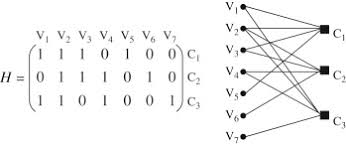
\includegraphics[width=0.7\textwidth]{./pic/Tanner Graph}}
    \caption{ Tanner Graph}
    \label{fig:Tanner Graph}
\end{figure}\cite{Tannerg} 

Die \autoref{fig:Tanner Graph} zeigt die variablen Knoten $V_j$  mit $j\in \left\{1, 2, 3, 4, 5, 6, 7\right\}$ und $C_k$ Prüfknoten mit $k\in \left\{1, 2, 3\right\}$.\\

\begin{Beispiel}[Der weiche Entscheidungsdekodieralgorithmus]
Angenommen, das Codewort $c$ wird gesendet und $y = c + e$ wird empfangen, wobei $e$ der unbekannte Fehlervektor ist. Angesichts des Syndroms $Hy^\intercal = He^\intercal = z^\intercal$ besteht das Ziel des dekodieres darin,\\ 

$prob(ek = 1 \mid z)$ für $1 \leq k \leq n$ zu berechnen.\\

Der Algorithmus berechnet iterativ zwei Wahrscheinlichkeiten für jede Kante des Tanner-Graphen und jedes $e\in \left\{0, 1\right\}$. 
Wenn der Graph Zyklen hat, sind diese Wahrscheinlichkeiten Annäherungen an\\

$prob(ek = 1 \mid z)$ für $1 \leq k \leq n$.\\

Letzten Endes ist es egal, wie diese Wahrscheinlichkeiten genau lauten; es geht nur darum, eine Lösung für $He^\intercal = z^\intercal$ zu erhalten.
Daher kann der Algorithmus auch dann erfolgreich eingesetzt werden, wenn lange Zyklen vorhanden sind.\cite[S. 11]{huffman}\\
\end{Beispiel}

% ----------------------------
\section{Vergleich von LDPC-Codes gegenüber herkömmlichen Blockcodes} 
% ----------------------------

\begin{Beispiel}[Vergleich von LDPC-Codes gegenüber herkömmlichen Blockcodes]

Bei LDPC - Codes werden, wie bei allen Blockcodes, den informationstragenden Bits zusätzliche Bits hinzugefügt. 
Diese zusätzlichen Bits, die als Paritätsbits bezeichnet werden, bilden zusammen mit den Informationsbits Paritätsgleichungen. 
Bei einer fehlerfreien Übertragung müssen diese Gleichungen bei einer  Paritätsprüfung null ergeben, dargestellt durch $Hc^\intercal=0$.\\

Ein Unterschied zu traditionellen Blockcodes liegt in der Dekodierungsmethode.
Klassische Blockcodes werden in einem einzigen Durchlauf dekodiert, während LDPC-Codes iterative Verfahren nutzen.\\

Ein zusätzlicher Unterschied ist, dass LDPC-Codes durch ihre Kontroll- Paritätsprüfmatrix charakterisiert sind und nicht, wie bei herkömmlichen Blockcodes, durch ihre Generatormatrix.
\end{Beispiel}

    